\documentclass[11pt]{article}
\RequirePackage{fullpage}
\RequirePackage[font=small,labelfont=bf]{caption}
\RequirePackage{amsmath,amssymb,amsthm}
\RequirePackage{mathtools}
\RequirePackage{graphicx}
\RequirePackage[normalem]{ulem}
\RequirePackage[hidelinks]{hyperref}
\RequirePackage{wrapfig}
\RequirePackage{subcaption}
\RequirePackage{authblk}
\RequirePackage{bm}
\RequirePackage{bbm}
\RequirePackage{tikz}


% line numbers:
\RequirePackage{lineno}
%\modulolinenumbers[5]
\renewcommand\linenumberfont{\normalfont\tiny\sffamily\color{black}}

% spacing
\RequirePackage{setspace}
%\doublespacing
 
% \RequirePackage[osf]{mathpazo}
\RequirePackage[bibstyle=authoryear,citestyle=authoryear-comp,
                date=year,
                maxbibnames=9,maxnames=5,maxcitenames=2,
                backend=biber,uniquelist=false,uniquename=false,
                % style=apa,
                sorting=nyt,
                hyperref=true]{biblatex}
\RequirePackage[colorinlistoftodos]{todonotes}  %disable
\RequirePackage{color}
\RequirePackage{nicefrac}

\newcommand{\gc}[1]{{\it \color{red} #1 } }
\newcommand{\vb}[1]{{\it \color{blue} #1}}
\newcommand{\vbout}[1]{{\it \color{blue} \sout{#1}}}

% a /nonumber you can turn on/off
\newcommand{\nnn}{\nonumber}
%\newcommand{\nnn}{}

\newcommand{\beginsupplement}{%
        \setcounter{table}{0}
        \renewcommand{\thetable}{S\arabic{table}}%
        \setcounter{figure}{0}
        \renewcommand{\thefigure}{S\arabic{figure}}%
     }


\newcommand{\graham}[1]{\todo[size=\scriptsize, color=red!50]{#1}}
\newcommand{\vince}[1]{\todo[size=\scriptsize, color=blue!50]{#1}}

\renewcommand{\P}{\mathbb{P}}
\newcommand{\E}{\mathbb{E}}
\newcommand{\V}{\text{V}}
\newcommand{\cf}{\emph{cf.} }
\DeclareMathOperator{\var}{Var}
\DeclareMathOperator{\cov}{Cov}
\DeclareMathOperator{\flt}{\mathrm{flat}}
\DeclareMathOperator{\T}{{\mathrm{T}}}
\newcommand{\vect}[1]{\mathbf{#1}}
\newcommand{\nssh}{SSH_n}

\newcommand{\chapquote}[2]{\begin{quotation} \textit{#1} \end{quotation} \begin{flushright} - #2\end{flushright} }

\addbibresource{biblio.bib}

% TODO
% - sig impact
% - ref table 1
% - more correction plots?
% - mention PCA



\title{Estimating the genome-wide contribution of selection to temporal allele frequency change}

% Significant Statement:

% A long-standing problem in evolution biology is to understand the different
% processes that shape the genetic composition of populations. In a population
% closed to migrants, the two processes that change the frequencies of alleles
% are selection, which systematically increases beneficial alleles and removes
% disadvantageous ones, and genetic drift which stochastically changes allele
% frequencies as some parents have more or less copies of specific
% alleles to the next generation. Previous efforts to
% disentangle these two processes have often used population genomic samples from a
% single timepoint and specific models of how selection at one allele affects its
% neighbors (known as linked selection). Here, we use genomic data taken at
% multiple timepoints to directly quantify how selection and drift change allele
% frequency change at a genome-wide level through time. We show selection acts
% over short timescales in three evolve-and-resequence studies and has a sizeable
% impact on genome-wide allele frequency changes. 


\author[$\ast$,$\dag$,$1$]{Vince Buffalo}
\author[$\dag$]{Graham Coop}
\affil[$\ast$]{\footnotesize Population Biology Graduate Group}
\affil[$\dag$]{\footnotesize Center for Population Biology, Department of Evolution and Ecology, University of California, Davis, CA 95616}
\affil[$1$]{\footnotesize Email for correspondence: \href{mailto:vsbuffalo@ucdavis.edu}{vsbuffalo@ucdavis.edu}}

\begin{document}
\maketitle

\linenumbers

\begin{abstract}

 Rapid phenotypic adaptation is often observed in natural populations and
 selection experiments.  However, detecting the genome-wide impact of this
 selection is difficult, since adaptation often proceeds from standing
 variation and selection on highly polygenic traits, both of which may leave
 faint genomic signals indistinguishable from a noisy background of genetic
 drift.  One promising signal comes from the genome-wide covariance between
 allele frequency changes observable from temporal genomic data, e.g.
 evolve-and-resequence studies. These temporal covariances reflect how the
 change in neutral allele frequency at one timepoint is predictive of the
 changes at later timepoints when there is heritable fitness variation in the
 population, as neutral alleles can remain associated with selected alleles
 over time. Since genetic drift does not lead to temporal covariance, we can
 use these covariances to estimate what fraction of the variation in allele
 frequency change through time is driven by linked selection. Here, we
 reanalyze \vb{three selection experiments}, \vbout{two \emph{Drosophila
   simulans} evolve-and-resequence studies, and one artificial selection
 experiment in mice}, to quantify the effects of linked selection over short
 timescales using covariance among time-points and across replicates. We
 estimate that at least 17\% to 37\% of allele frequency change is driven by
 selection in these experiments.  Against this background of positive
 genome-wide temporal covariances we also identify signals of negative temporal
 covariance corresponding to reversals in the direction of selection for a
 reasonable proportion of loci over the time course of a selection experiment.
 Overall, we find that in the three studies we analyzed, linked selection has a
 large impact on short-term allele frequency dynamics that is readily
 distinguishable from genetic drift.

\end{abstract}

\subsubsection*{Significant Statement}

A long-standing problem in evolution biology is to understand the different
processes that shape the genetic composition of populations. In a population
closed to migrants, the two processes that change \vb{allele frequencies} are
selection, which systematically increases beneficial alleles and removes
\vb{deleterious} ones, and genetic drift which stochastically changes allele
frequencies as some parents have more or less copies of specific alleles to the
next generation. Previous efforts to disentangle these two processes have often
used population genomic samples from a single timepoint and specific models of
how selection at one allele affects its neighbors (known as linked selection).
Here, we use genomic data taken at multiple timepoints to \vbout{directly}
quantify \vb{the relative contributions of} selection and drift \vb{to} allele
frequency \vb{changes} at a genome-wide level through time. We show selection acts
over short timescales in three evolve-and-resequence studies and has a sizeable
impact on genome-wide allele frequency changes. 




\section{Introduction}

A long-standing problem in evolutionary genetics is quantifying the roles of
genetic drift and selection in shaping genome-wide allele frequency changes.
Selection can affect allele frequencies, \vb{both directly and indirectly,}
with the indirect effect coming from the action of selection on \vb{linked}
loci elsewhere in genome e.g. linked selection (\cite{Maynard_Smith1974-lc},
\cite{Charlesworth1993-gb,Nordborg1996-nq}; see \cite{Barton2000-zg} for a
review). Previous work \vbout{on this question} has mostly focused on teasing
apart the impacts of drift and selection on genome-wide diversity using
population samples from a single contemporary timepoint, often by modeling the
correlation between regional recombination rate, gene density, and diversity
created in the presence of linked selection
\parencite{Cutter2013-ba,Sella2009-nx}. This approach has shown linked
selection has a major role in shaping patterns of genome-wide diversity across
the genomes of a range of sexual species
\parencite{Macpherson2007-qt,Andolfatto2007-uy,Begun2007-bg,Beissinger2016-cm,Sattath2011-dr,Williamson2014-oy,Andersen2012-bj,Cutter2010-gi,Elyashiv2016-vt},
and has allowed us to quantify the relative influence of positive selection
(hitchhiking) and negative selection (background selection;
\cite{Nordborg2005-dc,McVicker2009-ax,Andolfatto2007-uy,Macpherson2007-qt,Hernandez2011-gs,Elyashiv2016-vt}).
However, we lack an understanding of how genome-wide linked selection acts over
time.

There are numerous examples of rapid phenotypic adaptation
\parencite{Grant2011-wk,Grant2006-hj,Reznick1997-mh,Franks2007-dr} and rapid,
selection-driven genomic evolution in asexual populations
\parencite{Good2017-om,Bennett1990-bc,Baym2016-kh}.  Yet the polygenic nature
of fitness makes detecting the impact of selection on genome-wide variation
over short timescales in sexual populations remarkably difficult
\vb{\parencite{Latta1998-me, Pritchard2010-tk,Kemper2014-bx}}. This is because
the effect of selection on a polygenic trait (such as fitness) is distributed
across loci in proportion to their effect sizes. This can lead to subtle allele
frequency shifts on standing variation that are difficult to distinguish from
background levels of genetic drift and sampling variance.  However,
increasingly genomic experimental evolution studies with multiple timepoints,
and in some cases multiple replicate populations, are being used to detect
large effect selected loci \parencite{Turner2011-sx,Turner2012-bm} and
differentiate modes of selection
\parencite{Burke2010-tz,Barghi2019-qy,Therkildsen2019-zy}.  In addition these
temporal-genomic studies have begun in wild populations, some with the goal of
finding variants that exhibit frequency changes consistent with fluctuating
selection \parencite{Bergland2014-ij,Machado2018-cs}. In a previous paper, we
proposed that one useful signal for understanding the genome-wide impact of
polygenic linked selection detectable from genomic studies with multiple
timepoints is the temporal autocovariance in allele frequency changes
\parencite{Buffalo2019-io}.  These covariances are directly estimable from
temporal genomic data and are created when the loci that underly heritable
fitness variation perturb the frequencies of linked neutral alleles; in
contrast, when genetic drift acts alone in a closed population, these
covariances are zero in expectation.  Mathematically, temporal covariances are
useful because it is natural to decompose the total variance in allele
frequency change across a set of time intervals into the variances and
covariances in allele frequency change among time intervals. Furthermore,
biologically, these covariances reflect the extent to which neutral allele
frequency changes in one generation predict changes in another due to a shared
selection pressures and associations to selected loci.

Here, we provide the first empirical analyses to quantify the impact of linked
selection acting over short timescales (tens of generations) across two evolve
and re-sequence studies \parencite{Barghi2019-qy,Kelly2019-dc}, and an
artificial selection experiment \parencite{Castro2019-uk}. We repeatedly find a
signal of temporal covariance, consistent with linked selection acting to
significantly perturb genome-wide allele frequency changes across the genome in
a manner that other approaches would not be able differentiate from genetic
drift. We estimate the lower bound on the proportion of total variation in
allele frequency change caused by selection, and the correlation between allele
frequency changes between replicate populations caused by the response to
convergent selection pressures. Overall, we demonstrate that linked selection
has a powerful role in shaping genome-wide allele frequency changes over very
short timescales.

\section{Results}

\begin{table}
  \centering
  \footnotesize
  \centering
  \begin{tabular}{l c c c c c c}
    \textbf{Study} & \textbf{Species} & \textbf{Selection} & \textbf{Replicates} & \textbf{Pop. Size} & \textbf{Gens.} & \textbf{Timepoints} \\ 
  \hline
    \textcite{Kelly2019-dc}  & \emph{D. simulans} & lab adaptation & 3 & $\sim$1100 & 14 & 2 \\ \hline
    \textcite{Barghi2019-qy} & \emph{D. simulans} & lab adaptation & 10 & $\sim$1000 & 60 & 7 \\ \hline
    \textcite{Castro2019-uk} & \emph{M. musculus} & \begin{tabular}{c}tibiae length\\control\end{tabular} & \begin{tabular}{c}2\\1\end{tabular} &\begin{tabular}{c}32\\28\end{tabular}  & 17 & 2 \\
 \hline
  \end{tabular}
  \caption{A summary of the main selection studies we analyzed.}
\end{table}

We first analyzed \textcite{Barghi2019-qy}, an evolve-and-resequence study with
ten replicate populations exposed to a high temperature lab environment and
evolved for 60 generations, and sequenced every ten generations. Using the
seven timepoints and ten replicate populations, we estimated the genome-wide $6
\times 6$ temporal covariance matrix $\mathbf{Q}$ for each of the ten
replicates. Each row of these matrices represent the temporal covariance
$\cov(\Delta_{_{10}} p_s, \Delta_{_{10}} p_t)$, between the allele frequency
change (in ten-generation intervals, denoted $\Delta_{_{10}} p_t$) in some
initial reference generation $s$ (the row of the matrix), and some later
timepoint $t$ (the column of the matrix). We corrected these matrices for
biases created due to sampling noise, and normalize the entries for
heterozygosity (see Supplementary Materials Sections
\ref{supp:ind-depth-var-corr} and \ref{supp:matrix-correction}). These
covariances are expected to be zero when only drift is acting, as only
heritable variation for fitness can create covariance between allele frequency
changes in a closed population \parencite{Buffalo2019-io}.  Averaging across
the ten replicate temporal covariances matrices, we find temporal covariances
that are statistically significant (95\% block bootstraps CIs do not contain
zero), consistent with linked selection perturbing genome-wide allele frequency
changes over very short time periods. The covariances between all adjacent time
intervals are positive and then decay towards zero as we look at more distant
time intervals (Figure \ref{fig:figure-1} A), as expected when directional
selection affects linked variants' frequency trajectories until ultimately
linkage disequilibrium and the additive genetic variance for fitness associated
with neutral alleles decays (\vb{which could occur as a population reaches
a new optimum}) \parencite{Buffalo2019-io}. The temporal covariances per
replicate are noisier but this general pattern holds; see Supplementary Figure
\ref{suppfig:barghi-cov-panels}.  \textcite{Barghi2019-qy}'s design means that
the covariances we see in adjacent time intervals are on average ten
generations apart, and given the temporal decay in covariance we see, the
covariances on shorter time-scales (e.g. if adjacent generations had been
sequenced) may well be higher yet (see Supplementary Material Section
\ref{supp:barghi-covs} for more details).

\vbout{One concern is that these covariances reflect the localized impact of a
  few large-effect loci rather than selection on a polygenic trait.} Since our
  covariances are essentially averages over loci, the covariance estimate \vb{could}
  be strongly affected by \vb{a few} outlier regions. To test whether large
  outlier regions drive the genome-wide signal we see in the
  \textcite{Barghi2019-qy} data, we calculate the covariances in 100kb windows
  along the genome (we refer to these as windowed covariances throughout) and
  take the median windowed covariance, and trimmed-mean windowed covariance, as
  a measure of the genome-wide covariance robust to large-effect loci. These
  robust estimates (Supplementary Table \ref{supp:table-trimmed-mean} and
  Supplementary Figure \ref{suppfig:barghi-trimmed-mean}) confirm the patterns
  we see using the mean covariance, confirming that genomic temporal
  covariances are non-zero due to the impact of selection acting across many
  genomic windows. 


\begin{figure}[!htb]
  \centering
  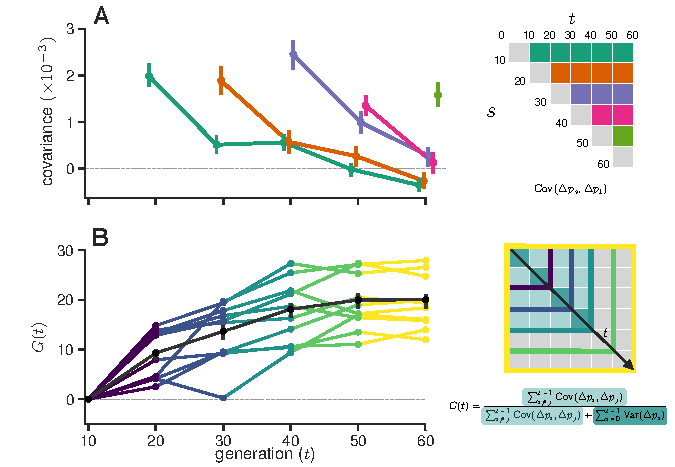
\includegraphics[width=\textwidth]{figures/figure-1-revision.pdf}

  \caption{A: Temporal covariance, averaged across all ten replicate
    populations, through time from the \textcite{Barghi2019-qy} study. Each
    line depicts the temporal covariance $\cov(\Delta p_s, \Delta p_t)$ from
    some reference generation $s$ to a later time $t$ which varies along the
    x-axis; each line corresponds to a row of the upper-triangle of the
    temporal covariance matrix with the same color (upper right). The ranges
    around each point are $95\%$ block-bootstrap confidence intervals. B: The
    proportion of the total variance in allele frequency change explained by
    linked selection, $G(t)$, as it varies through time $t$ along the x-axis.
    The black line is the $G(t)$ averaged across replicates, with the $95\%$
    block-bootstrap confidence interval. The other lines are the $G(t)$ for
    each individual replicate, with colors indicating what subset of the
    temporal-covariance matrix to the right is being included in the
  calculation of $G(t)$.}

  \label{fig:figure-1}
\end{figure}

While the presence of positive temporal covariances is consistent with
selection affecting allele frequencies over time, this measure is not easily
interpretable. We can calculate a more intuitive measure from the temporal
covariances to quantify the impact of selection on allele frequency change: the
ratio of total covariance in allele frequency change to the total variance in
allele frequency change. We denote the change in allele frequency as $\Delta
p_t = p_{t+1}-p_t$, where $p_t$ is the allele frequency in generation $t$.
Since the total variation in allele frequency change can be partitioned into
variance and covariance components, $\var(p_t - p_0) = \sum_{i=0}^{t-1}
\var(\Delta p_i) + \sum_{i \ne j}^{t-1} \cov(\Delta p_i, \Delta p_j)$ (we bias
correct these for sequencing depth), and the covariances are zero when drift
acts alone, this is a lower bound on how much of the variance in allele
frequency change is caused by linked selection \parencite{Buffalo2019-io}. We
call this measure $G(t)$, defined as

\begin{align}
  G(t) = \frac{\sum_{i\ne j}^{t-1} \cov(\Delta p_i, \Delta p_j)}{\var(p_t - p_0)}
\end{align}
%
which estimates the effect of selection on allele frequency change between the
initial generation $0$ and some later generation $t$, which can be varied to
see how this quantity grows through time. Since \textcite{Barghi2019-qy}
experiment is sequenced every ten generations, in the numerator for the
covariance we use the allele frequency changes between adjacent timepoints,
which are ten generations apart. Consequently, this leads our measure $G(t)$ to
be strongly conservative, since the temporal covariances within each
ten-generation block are not directly observable, and thus are not included in
the numerator of $G(t)$. Still, we find a remarkably strong signal. Greater
than $20\%$ of total, genome-wide allele frequency change over 60 generations
is the result of selection (Figure \ref{fig:figure-1} B).

Additionally, we looked for a signal of temporal autocovariance in
\textcite{Bergland2014-ij}, a study that collected \emph{Drosophila
melanogaster} through Spring-Fall season pairs across three years. If there was
a strong  pattern of genome-wide fluctuating selection, we might expect a
pattern of positive covariances between similar seasonal changes, e.g.
Spring-Fall in two adjacent years, and negative covariances between dissimilar
seasonal changes, e.g. Spring-Fall and Fall-Spring in two adjacent years.
However, we find no such signal over years, \vb{and in reproducing their
  original analysis, we find that their number of statistically significant
  seasonal SNPs is not enriched compared to an empirical null distribution
  created by permuting seasonal labels}; we discuss this in more depth in
  Supplementary Materials Section \ref{supp:bergland-reanalysis}.

The replicate design of \textcite{Barghi2019-qy} allows us to quantify another
covariance: the covariance in allele frequency change between replicate
populations experiencing convergent selection pressures. These
between-replicate covariances are created in the same way as temporal
covariances: neutral alleles linked to a particular fitness background are
expected to have allele frequency changes in the same direction if the
selection pressures are similar. Intuitively, where temporal covariances
reflect that neutral alleles associated with heritable fitness backgrounds are
predictive of frequency changes between generations, replicate covariances
reflect that heritable fitness backgrounds common to each replicate predict
(under the same selection pressures) frequency changes between replicates. We
measure this through a statistic similar to a correlation, which we call the
convergent correlation: the ratio of average between-replicate covariance
across all pairs to the average standard deviation across all pairs of
replicates, 


\begin{align}
  \label{eq:conv-corr}
  \mathrm{cor}(\Delta p_s, \Delta p_t) = \frac{\E_{A\ne B} \left( \cov(\Delta p_{s,A}, \Delta p_{t,B}) \right)}{\E_{A\ne B} \left( \sqrt{\var(\Delta p_{s,A}) \var(\Delta p_{t,B})} \right)}
\end{align}
%
where $A$ and $B$ here are two replicate labels, and for the
\textcite{Barghi2019-qy} data, we use $\Delta_{_{10}} p_t$.

We've calculated the convergent correlation for all rows of the replicate
covariance matrices. Like temporal covariances, we visualize these through time
(Figure \ref{fig:figure-2} A), with each line representing the convergent
correlation from a particular reference generation $s$ as it varies with $t$
(shown on the x-axis). In other words, each of the colored lines corresponds to
the like-colored row of the convergence correlation matrix (upper left in
Figure \ref{fig:figure-2} A). We find these convergent covariances are
relatively weak, and decay very quickly from an initial value of about 0.1
(95\% block bootstrap confidence intervals $[0.094, 0.11]$) to around 0.01
(95\% CIs [0.0087, 0.015]) within 20 generations. This suggests that while
a reasonable fraction of the initial response is shared over the replicates,
this is followed by a rapid decay, a result consistent with the primary
finding of the original \textcite{Barghi2019-qy} study: that alternative loci
contribute to longer term adaptation across the different replicates. 

\begin{figure}[!htb]
  \centering
  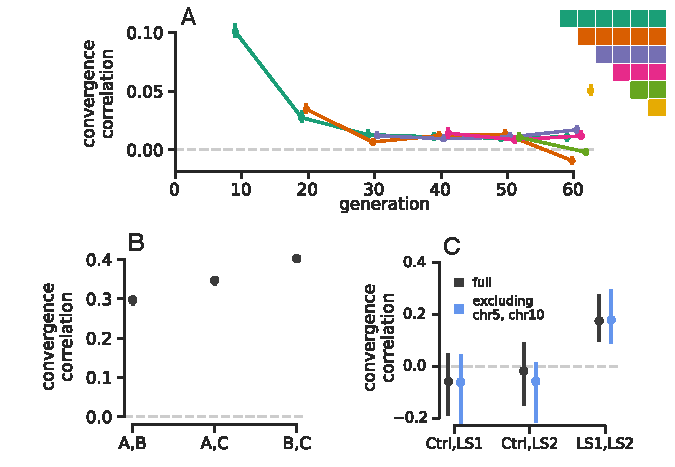
\includegraphics[width=\textwidth]{figures/figure-2-revision.pdf}

  \caption{{\bf A}: The convergence \vb{correlations}, averaged across
    \textcite{Barghi2019-qy} replicate pairs, through time. Each line
    represents the convergence correlation $\mathrm{cor}(\Delta p_{s}, \Delta
    p_{s})$ from a starting reference generation $s$ to a later time $t$, which
    varies along the x-axis; each line corresponds to a row of the temporal
    convergence correlation matrix depicted to the right. We note that
    convergent correlation for the last timepoint is an outlier; we are unsure
    as to the cause of this, e.g. it does not appear to be driven by a single
    pair of replicates. {\bf B}: The convergence \vb{correlations} between
    individual pairs of replicates in the \textcite{Kelly2019-dc} data
    (\vb{note the confidence intervals are plotted, but are small on this
    y-axis scale; see note XXX}). {\bf C}:  The convergence \vb{correlations}
    between individual pairs of replicates in \parencite{Castro2019-uk} data,
    for the two selection lines  (LS1 and LS2) and the control (Ctrl); gray CIs
    are those using the complete dataset, blue CIs exclude chromosomes 5 and 10
    which harbor the two regions \textcite{Castro2019-uk} found to have signals
  of parallel selection between LS1 and LS2.}

  \label{fig:figure-2}
\end{figure}

A benefit of between-replicate covariances is that unlike temporal covariances,
these can be calculated with only two sequenced timepoints and a replicated
study design. This allowed us to assess the impact of linked selection in
driving convergent patterns of allele frequency change across replicate
populations in two other studies. First, we reanalyzed the selection experiment
of \textcite{Kelly2019-dc}, which evolved three replicate wild populations of
\emph{Drosophila simulans} for 14 generations adapting to a novel laboratory
environment. Since each replicate was exposed to the same selection pressure
and share linkage disequilibria common to the original natural founding
population, we expected each of the three replicate populations to have
positive between-replicate covariances. We find all three pairwise
between-replicate covariances are positive and statistically significant
(Figure \ref{fig:figure-2} B. We estimate the convergent correlation
coefficient across these replicates as 0.36 ($95\%$ CI $[0.31, 0.40]$).
Similarly, we can calculate the proportion of the total variance in allele
frequency change from convergent selection pressure analogous to $G$ where the
numerator is is the convergent covariance and the denominator is the total
variance (see Supplementary Material \ref{supp:replicate-g}). We find that 37\%
of the total variance is due to shared allele frequency changes caused by
selection (95\% CI [29\%, 41\%]; these are similar to the convergence
correlation, since the variance is relatively constant across the replicates.

% 95\% CIs, [0.00635, 0.00860], [0.00636, 0.00859], [0.00608, 0.00834])

Next, we reanalyzed the Longshanks selection experiment, which selected for
longer tibiae length relative to body size in mice, leading to a response to
selection of about 5 standard deviations over the course of twenty generations
\parencite{Marchini2014-de,Castro2019-uk}. This study includes two independent
selection lines, Longshanks 1 and 2 (LS1 and LS2), and an unselected control
line (Ctrl).  Consequently, this selection experiment offers a useful control
to test our between-replicate covariances: we expect to see positive
between-replicate covariance in the comparison between the two Longshanks
selection lines, but not between the two pairwise comparisons between the
control line and each of the two Longshanks lines. We find that this is
the case (gray confidence intervals in Figure \ref{fig:figure-2} C), with the
two Longshanks comparisons to the control line not being significantly
different from zero, while the comparison between the two Longshanks lines is
statistically significantly different from zero (CIs [0.0129, 0.0400]).

One finding in the Longshanks study was that two major-effect loci showed
parallel frequency shifts between the two selection lines: a region harboring
the gene Nkx3-2 known to be involved in limb development, and another region
containing six other candidate genes. We were curious to what extent our
genome-wide covariances were being driven by these two outlier large-effect
loci, so we excluded them from the analysis. Since we do not know the extent to
which linkage disequilibrium around these large-effect loci affects neighboring
loci, we took the conservative precaution of excluding the entire chromosomes
these loci reside on (chromosomes 5 and 10), and re-calculating the temporal
covariances. We find excluding these large effect loci has little impact on the
confidence intervals (blue confidence intervals in Figure \ref{fig:figure-2} C),
indicating that these across-replicate covariances are indeed driven by a large
number of loci. This is consistent with a signal of selection on a polygenic
trait driving genome-wide change, although we note that large-effect loci can
contribute to the indirect change at unlinked loci
\parencite{Robertson1961-ho,Santiago1995-hx}. 

The presence of an unselected control line provides an alternative way to
partition the effects of linked selection and genetic drift: we can compare the
total variance in allele frequency change of the control line (which excludes
the effect of artificial selection on allele frequencies) to the total variance
in frequency change of the Longshanks selection lines. This allows us to
estimate the increase in variance in allele frequency change due to selection,
which we can further partition into the effects of selection shared between
selection lines and those unique to a selection line by using estimating the
shared effect through the observed covariance between replicates (see Materials
and Methods \ref{sec:mm-partition} and Supplementary Material Section
\ref{supp:replicate-g} for more details).  We estimate at least 32\% (95\% CI
$[21\%, 48\%]$) of the variance in allele frequency change is driven by the
effects of selection, of which 14\% (95\% CI $[3\%, 33\%]$) is estimated to be
unique to a selection line, and 17\% (95\% CI $[9\%, 23\%]$) is the effect of
shared selection between the two Longshanks selection lines (and the value of
the convergence correlation between the Longshanks lines, a related statistic,
is 0.18, 95\% CI [0.0743, 0.254]).

% We can partition the
% allele frequency change between the two timepoints (20 generations apart) for a
% Longshanks line as $\Delta p_{t,\mathrm{LS1}} = \Delta_{_{D}}
% p_{t,\mathrm{LS1}} + \Delta_{_{U}} p_{t,\mathrm{LS1}} + \Delta_{_S}
% p_{t,\mathrm{LS}}$ where these terms are the decomposition in the allele
% frequency change due to drift in Longshanks replicate 1 ($\Delta_{_D}
% p_{t,\mathrm{LS1}}$), selection unique to the LS1 replicate ($\Delta_{_U}
% p_{t,\mathrm{LS1}}$), and selection response shared between the two Longshanks
% replicates ($\Delta_{_S} p_{t,\mathrm{LS}}$) respectively (and similarly for
% the Longshanks two line, LS2). By construction we will assume that each of
% these terms are uncorrelated within replicates, and that only the shared term
% covaries between the replicates.  Assuming that we can approximate the
% contribution of genetic drift in the LS lines as the variance in allele
% frequency change observed in the control, i.e.  $\var(\Delta
% p_{t,\mathrm{Ctrl}}) = \var(\Delta_{_{D}}
% p_{t,\mathrm{LS2}})=\var(\Delta_{_{D}} p_{t,\mathrm{LS2}})$, then we can
% estimate the increase in variance in allele frequency change due to selection
% as $(\var(\Delta p_{t,\mathrm{LS1}}) + \var(\Delta p_{t,\mathrm{LS2}}))/2 -
% \var(\Delta p_{t,\mathrm{Ctrl}})$ and the shared effect of selection across
% selected lines as $\cov(\Delta p_{t,\mathrm{LS1}}, \Delta p_{t,\mathrm{LS2}})$



\begin{figure}
  \centering
  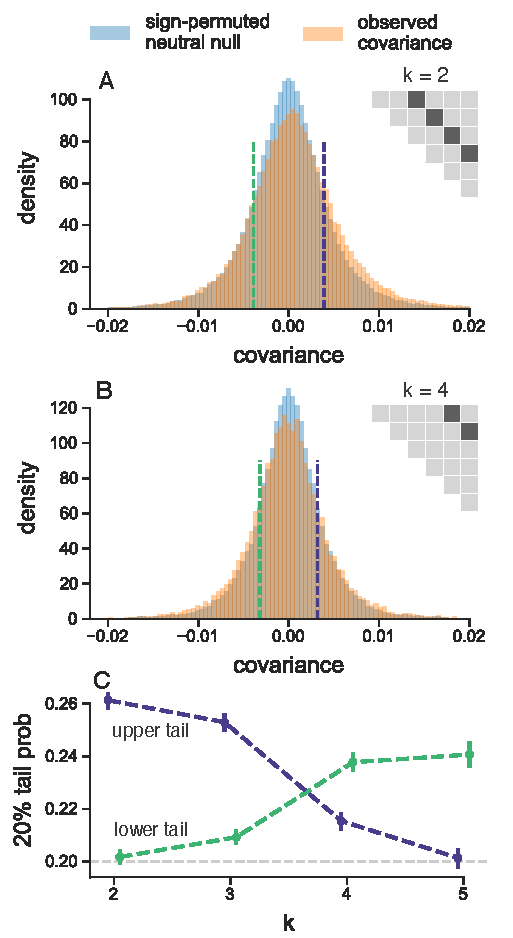
\includegraphics[]{figures/figure-3-revision.pdf}

  \caption{\footnotesize {\bf A}, {\bf B}: The distribution of temporal
    covariances calculated in 100kb genomic windows from the
    \textcite{Barghi2019-qy} study, plotted alongside an empirical neutral null
    distribution created by recalculating the windowed covariances on 1,000
    sign permutations of allele frequency changes within tiles. The histogram
    bin number is 88, chosen by cross validation (Supplementary Materials
    \ref{suppfig:barghi-cross-validation-binsize}). In subfigure {\bf A},
    windowed covariances $\cov(\Delta p_t, \Delta p_{t+k})$ are separated by
    $k=2 \times 10$ generations and in subfigure {\bf A} the covariances are
    separated by $k=4 \times 10$ generations; each $k$ is an off-diagonal from
    the variance diagonal of the temporal covariance matrix (see cartoon of
    upper-triangle of covariance matrix in subfigures {\bf A} and {\bf B},
    where the first diagonal is the variance, and the dark gray indicates which
    off-diagonal of the covariance matrix is plotted in the histograms). {\bf
    C}: The lower and upper tail probabilities of the observed windowed
    covariances, at 20\% and 80\% quintiles of the empirical neutral null
    distribution, for varying time between allele frequency changes (i.e. which
    off-diagonal $k$). The confidence intervals are  $95\%$ block-bootstrap
  confidence intervals, and the light gray dashed line indicates the 20\% tail
probability expected under the neutral null. Similar figures for different
values of $k$ are in Supplementary Figures
\ref{suppfig:barghi-empnull-tilecovs}. }

    \label{fig:figure-3} 
\end{figure}


Finally, we observed that in the longest study  we analyzed
\parencite{Barghi2019-qy}, some genome-wide temporal covariances become
negative at future timepoints (see the first two rows in Figure
\ref{fig:figure-1} A). This shows that alleles that were on average going up
initially are later going down in frequency, i.e. that the average direction of
selection experienced by alleles has flipped. This must reflect either a change
in the environment or the genetic background, due to epistatic relationships
among alleles altered by frequency changes or recombination breaking up
selective alleles.  Such reversals of selective dynamics could be occurring at
other timepoints but the signal of a change in the direction of selection at
particular loci may be washed out when we calculate our genome-wide average
temporal covariances. To address this limitation, we calculated the
distribution of the temporal covariances over 100kb windowed covariances
(Figure \ref{fig:figure-3} shows these distributions pooling across all
replicates; see Supplementary Figure
\ref{suppfig:barghi-offset-replicate-panels} for individuals replicates). The
covariance estimate of each genomic window will be noisy, due to sampling and
genetic drift, and the neutral distribution of the covariance is complicated
due to linkage disequilibria (which can occur over long physical distances in
E\&R and selection studies, \cite{Nuzhdin2013-gf,Baldwin-Brown2014-cl}). To
address this, we have developed a permutation-based procedure that constructs
an empirical null distribution by randomly flipping the signs of the allele
frequency changes per-genomic window. This destroys the systematic covariances
created by linked selection and creates a sampling distribution of the
covariances spuriously created by neutral genetic drift while preserving the
complex dependencies between adjacent loci created by linkage disequilibrium.
This empirical neutral null distribution is conservative in the sense that the
variances of the covariances are wider than expected under drift alone as they
include the effect of selection on the allele frequency change within a
time-interval, just not between time-intervals. We see (Figure
\ref{fig:figure-3} A and B) that windowed temporal covariances between close
timepoints are skewed positive (a heavy right tail), while between more distant
timepoints these windowed temporal covariances tend to shift to become more
negative (a heavy left tail).  We quantified the degree to which the left and
right tails are inflated compared to the null distribution as a function of
time, and see excesses in both tails in Figure \ref{fig:figure-3} C. This
finding is also robust to sign-permuting allele frequency changes on a
chromosome-level, the longest extent that gametic linkage disequilibria can
extend (Supplementary Figure \ref{suppfig:barghi-tailprobs-seqid}). We see a
striking pattern that the windowed covariances not only decay towards zero, but
in fact become negative through time, consistent with many regions in the
genome having had a reversed fitness effect at later timepoints.

\section{Discussion}

Since the seminal analysis of \textcite{Maynard_Smith1974-lc} demonstrating
that linked neutral diversity is reduced as an advantageous polymorphism arises
and sweeps to fixation, over four decades of theoretical and empirical research
has enriched our understanding of linked selection.  One under-used approach to
understand the genome-wide effects of selection on standing variation, e.g.
selection on an infinitesimal polygenic trait, stems from an early quantitative
genetic model of linked selection \parencite{Robertson1961-ho} and its later
developments
(\cite{Santiago1995-hx,Santiago1998-bs,Wray1990-zf,Woolliams1993-qo}; see also
\cite{Barton2000-zg} for a comparison of these models with classic hitchhiking
models). Implicit in these models is that autocovariance between allele
frequency change is created when there is heritable fitness variation in the
population, a signal that may be readily detected from temporal genomic data
\parencite{Buffalo2019-io}.  Depending on how many loci affect fitness, such a
strong effect of linked selection may not be differentiable from genetic drift
using only single contemporary population samples or looking at at temporal
allele frequency change at each locus in isolation.  In this way, averaging
summaries of temporal data allows us to sidestep the key problem of detecting
selection from standing variation: that the genomic footprint leaves too soft
of a signature to differentiate from a background of genetic drift. In fact we
find that the temporal covariance signal is detectable even in the most
extremely difficult to detect soft sweep case: polygenic selection on highly
polygenic traits \parencite{Buffalo2019-io}.

It is worth building some intuition why temporal covariance allows us to detect
such faint signals of polygenic linked selection from temporal genomic data.
Each variant is subject to both variance in allele frequency due to drift and
sampling noise, which at any locus may swamp the temporal covariance signal and
creates spurious covariances. However, these spurious covariances do not share
a directional signal whereas the covariances created by linked selection do;
consequently, averaging across the entire genome, the temporal signal exceeds
sampling noise. 

Our analyses reveal that a sizable proportion of allele frequency change in
these populations is due to the (indirect) action of selection. Capitalizing on
replicated designs, we characterized the extent to which convergent selection
pressures lead to parallel changes in allele frequencies across replicate
populations, and found that a reasonable proportion of the response is shared
across short timescales. These likely represent substantial under-estimates of
the contribution of linked selection because the studies we have reanalyzed do
not sequence the population each generation, preventing us from including the
effects of stronger correlations between adjacent generations.  Furthermore,
our estimation methods are intentionally conservative, for example they exclude
the contribution of selection that does not persist across generations and
selection that reverses sign; thus they can be seen as a strong lower bound of
the effects of selection.

These estimates of the contribution of selection could be refined by using
patterns of LD and recombination which would allow us to more fully
parameterize a linked-selection model of temporal allele frequency change
\parencite{Buffalo2019-io}. The basic prediction is that regions of higher
linkage disequilibrium and lower recombination should have greater temporal
autocovariance than regions with lower LD and higher recombination. However,
one limitation of these pooled sequence datasets is that none of the studies we
reanalyzed estimated linkage disequilibria data for the evolved populations.
While there are LD data for a natural population of \emph{D. simulans}
\parencite{Signor2018-wg,Howie2018-ay},  we did not find a relationship between
temporal covariance and LD.  We believe this is driven by the idiosyncratic
nature of LD in evolve-and-resequence populations, which often extends over
large genomic distances \parencite{Nuzhdin2013-gf,Kelly2019-dc}. Future studies
complete with LD data and recombination maps would allow one to disentangle the
influence of closely linked sites from more distant sites in causing temporal
autocovariance, and allow the fitting of more parametric models to estimate
population parameters such as the additive genetic variation for fitness
directly from temporal genomic data alone \parencite{Buffalo2019-io}.

Our primary focus here has been on evolution in laboratory populations. It is
unclear whether we should expect a similar impact of selection in natural
populations. In some of these experiments, selection pressures may have been
stronger or more sustained that in natural populations
\parencite{Hendry1999-zu,Hairston2005-ga}. Conversely, these lab
populations were maintained at very small effective population sizes, estimated
at 300, 450, and 45 for the \textcite{Barghi2019-qy}, \textcite{Kelly2019-dc},
and \textcite{Castro2019-uk} studies respectively, which will amplify the role
of genetic drift. The advantage of lab experiments is that they are closed
populations, in natural populations temporal covariance could also arise from
the systematic migration of alleles from differentiated populations.
Adapting these methods to natural populations will require either
populations that are reasonably closed to migration, or for the effect of
migration to be accounted for possibly either by knowledge of allele
frequencies in source populations or the identification of migrant individuals. 

While it challenging to apply temporal methods to natural populations there is
a lot of promise for these approaches
\parencite{Bergland2014-ij,Machado2018-cs}. Efforts to quantify the impact of
linked selection have found obligately sexual organisms have up to an 89\%
reduction in genome-wide diversity over long time periods
\parencite{McVicker2009-ax,Elyashiv2016-vt,Corbett-Detig2015-gt,Coop2016-gx,Comeron2014-nh}
Thus linked selection makes a sizeable contribution to long-term allele
frequency change in some species, and there is reason to be hopeful that we
could detect this from temporal data, which would help to resolve the
timescales that linked selection act over. In our reanalysis of the
\textcite{Barghi2019-qy} study, we find evidence of complex linked selection
dynamics, with selection pressures flipping over time due to either
environmental change, the breakup of epistatic combinations or advantageous
haplotypes. Such patterns would be completely obscured in samples only from
contemporary populations. Thus, we can hope to have a much richer picture
of the impact of selection as temporal sequencing becomes more common,
allowing us to observe the effects of ecological dynamics in genomic data
\parencite{Hairston2005-ga}.

Furthermore, understanding the dynamics of linked selection over short
timescales will help to unite phenotypic studies of rapid adaptation with a
detectable genomic signature, to address long-standing questions concerning
linked selection, evolutionary quantitative genetics, and the overall impact
selection has on genetic variation. 

\section{Materials and Methods}

\subsection{Datasets Analyzed}

We used available genomic data data from four studies: pooled population
resequencing (pool-Seq) data from \textcite{Barghi2019-qy},
\textcite{Kelly2019-dc}, \textcite{Bergland2014-ij}, and
\textcite{Castro2019-uk}. In all cases, we used the variants kept after the
filtering criteria of the original studies. 

\subsection{Variance and Covariance Estimates}

To remove systematic covariances in allele frequency change caused by tracking
the reference or minor allele, we randomly choose which allele's frequency to
track for each locus. Then, we calculate the variance-covariance matrix of
allele frequency changes using a Python software package we have written,
available at \url{http://github.com/vsbuffalo/cvtk}. This simultaneously
calculates temporal variances and covariances, and replicate covariances and
uses the sampling depth and number of diploid individuals to correct for bias
in the variance estimates and a bias that occurs in covariance estimates
between adjacent timepoints due to shared sampling noise (see Supplementary
Material Sections \ref{supp:ind-depth-var-corr}, \ref{supp:cov-corr}, and
\ref{supp:matrix-correction} for mathematical details of these estimators). We
assess that our bias correction procedure is working adequately through a
series of diagnostic plots that ensure that the procedure removes the
relationship between sampling depth and uncorrected variance and covariances
(Supplementary Figure \ref{suppfig:bergland-correction}).


\subsection{Estimating Uncertainty with a Block Bootstrap}

To infer the uncertainty of covariance, convergence correlation, and $G(t)$
estimates, we used a block bootstrap procedure. This bootstrap procedure
resamples blocks of data points, rather than individual data points, to infer
the uncertainty of an statistic in the presence of unknown correlation between
loci. As most estimators in this paper are ratios (e.g. covariance standardize
by sample heterozygosity, $G(t)$, and the convergence correlation) which we
estimate with a ratio of averages, we exploit the linearity of expectation for
efficient computation of bootstrap samples (see \ref{supp:block-bootstrap} for
details).

\subsection{Partitioning Unique and Shared Selection Effects in the Longshanks Study}
\label{sec:mm-partition}

The unselected control line in the Longshanks experiment allows us to
additionally partition the total variance in allele frequency change into
drift, shared effects of selection, and unshared effects of selection between
selected replicates. We begin by decomposing the allele frequency change in
Longshanks line 1 (LS1) as $\Delta p_{t,\mathrm{LS1}} = \Delta_{_{D}}
p_{t,\mathrm{LS1}} + \Delta_{_{U}} p_{t,\mathrm{LS1}} + \Delta_{_S}
p_{t,\mathrm{LS}}$ where these terms are the drift in Longshanks replicate 1
($\Delta_{_D} p_{t,\mathrm{LS1}}$), selection unique to the LS1 replicate
($\Delta_{_U} p_{t,\mathrm{LS1}}$), and selection response shared between the
two Longshanks replicates ($\Delta_{_S} p_{t,\mathrm{LS}}$) respectively (and
similarly for the Longshanks line 2, LS2). By construction, this decomposition
assumes that each of these terms are uncorrelated within replicates, so the
contribution of each term to the total variance in allele frequency change,
$\var(\Delta p_{t,\mathrm{LS1}})$, is the variance in of that term's allele
frequency change. 

We estimate the effects of selection by first calculating the fraction of the
total variance explained by drift. We assume the variance in allele frequency
change observed in the unselected control line ($\var(\Delta
p_{t,\mathrm{Ctrl}})$) is driven entirely by neutral genetic drift, and since
an identical breeding scheme was used across all three replicates (except
breeders for the control line were chosen at random), we can use this as an
estimate of the contribution of neutral genetic drift in the selected lines,
$\var(\Delta p_{t,\mathrm{Ctrl}}) = \var(\Delta_{_{D}} p_{t,\mathrm{LS1}}) =
\var(\Delta_{_{D}} p_{t,\mathrm{LS2}})$. Then, we can estimate the increase in
variance in allele frequency change due to selection as $(\var(\Delta
p_{t,\mathrm{LS1}}) + \var(\Delta p_{t,\mathrm{LS2}}))/2 - \var(\Delta
p_{t,\mathrm{Ctrl}})$ and the shared effect of selection across selected lines
as $\cov(\Delta p_{t,\mathrm{LS1}}, \Delta p_{t,\mathrm{LS2}})$. Finally, the
covariance in allele change between replicates is used to estimate the shared
effects of selection between lines, $\cov(\Delta p_{t,\mathrm{LS1}}, \Delta
p_{t,\mathrm{LS2}}) = \var(\Delta_{_S} p_{t,\mathrm{LS}})$.

\subsection{Windowed Covariance and the Empirical Neutral Null}

Throughout the paper, we use genomic windows for the block-bootstrap procedure.
For the \emph{D. simulans} and \emph{D.  melanogaster} data from the
\textcite{Barghi2019-qy}, \textcite{Kelly2019-dc}, and
\textcite{Bergland2014-ij} studies, we used large megabase windows for the
block bootstrap procedure, while we used a ten megabase window for the large
mouse genome data from the \textcite{Castro2019-uk} study. 

Given evidence of a reversal in the direction of selection at later timepoints
in the \textcite{Barghi2019-qy} study, we calculated windowed temporal
covariances on 10 kilobase windows and looked at the distribution of these
covariances through time. We compare these distributions of windowed
covariances to an empirical neutral null created by randomly permuting the sign
of allele frequency change at the block level (to preserve the correlation
structure between loci due to LD). This destroys the systematic covariances in
allele frequency change created by linked selection, which emulates a frequency
trajectory under drift. This approach is conservative, since heritable fitness
variation also inflates the magnitude of allele frequency change more than
expected under drift, but we do not change these magnitudes. Using this
empirical neutral null distribution of windowed covariances, we calculate how
much of the observed windowed covariance distribution falls outside of
empirical null distribution for different tail probabilities. While the
comparison between the distribution of 10 kilobase windowed covariances to the
empirical neutral null created from sign-permuting 10 kilobase windows is most
natural, we wanted to ensure that our finding that the shift from mostly
positive to mostly negative windowed covariances through time (Figure
\ref{fig:figure-3}) was robust to LD extending beyond the range of these 10
kilobase windows. We took the conservative approach of also sign-permuting at
the chromosome-level, and found the same qualitative shift (Supplementary
Figure \ref{suppfig:barghi-tailprobs-seqid}).

\section{Acknowledgments} 

We would like to thank the authors of the original studies we've analyzed,
including Neda Barghi, Christian Schl{\"o}tterer, John Kelly, Kimberly Hughes,
Frank Chan, Campbell Rolian, Nick Barton, Alan Bergland, and Dmitri Petrov. We
would also like to thank Doc Edge for helpful statistical advice, and Matt
Osmond, Erin Calfee, Andy Kern, Sivan Yair, \vb{Chuck Langley, Dave Begun, and
Michael Turelli} for helpful discussions. \vb{Additionally, we thank Guy Sella
and one additional anonymous reviewer for greatly improving the manuscript}.
This research was supported by an NSF Graduate Research Fellowship grant
awarded to VB (1650042), and NIH (R01-GM108779) and NSF (1353380) awarded to
GC.



\printbibliography



\setcounter{section}{1}
\section*{Supplementary Material}
\beginsupplement

\subsection{Estimator Bias Correction}
\subsubsection{Correcting variance bias with a single depth sampling process}
\label{supp:depth-var-corr}

Following \textcite{Waples1989-sj}, we have that the variance in allele
frequency change at a locus in the initial generation, which is entirely due to
the binomial sampling process, is $\var(p_0) = \nicefrac{p_0(1-p_0)}{d_0}$
where $d_0$ is the number of binomial draws (e.g. read depth). At a later
timepoint, the variance in allele frequency is a result of both the binomial
sampling process at time $t$ and the evolutionary process. Using the law of
total variation we can partition the variation from each process,

\begin{align}
  \var(\widetilde{p_t}) &= \E(\var(\widetilde{p_t} | p_t)) + \var(\E(\widetilde{p_t}|p_t)) \\
                        &= \underbrace{\frac{p_t(1-p_t)}{d_t}}_\text{generation $t$ sampling noise} + \underbrace{\var(p_t)}_\text{variance due to evolutionary process}.
  %\frac{\var(\widetilde{p_t})}{p_0(1-p_0)} &= \frac{p_t(1-p_t)}{p_0(1-p_0) d_t} + 1 - \left( 1-\frac{1}{2N}\right)^t.
  %\frac{\var(\widetilde{p_t})}{p_0(1-p_0)} &= \frac{p_t(1-p_t)}{p_0(1-p_0) d_t} + \frac{t}{2N} + O\left((2 N)^{-2}\right).
\end{align}

Under a drift-only process, $\var(p_t) = p_0(1-p_0)\left[1- \left(1 -
\frac{1}{2N}\right)^t\right]$. However, with heritable variation in fitness, we
need to consider the covariance in allele frequency changes across generations
\parencite{Buffalo2019-io}. We can write

\begin{align}
  \var(p_t) &= \var\left(p_0 + (p_1 - p_0) + (p_2 - p_1) + \ldots + (p_t - p_{t-1}) \right) \\
         &= \var\left(p_0 + \Delta p_0 + \Delta p_1 + \ldots + \Delta p_{t-1} \right) \\
         &= \var(p_0) + \sum_{i=0}^{t-1} \cov(p_0, \Delta p_i) + \sum_{i=0}^{t-1} \var(\Delta p_i) + \sum_{0 \le i < j}^{t-1} \cov(\Delta p_i, \Delta p_j).
\end{align}
%

Each allele frequency change is equally like to be positive as it is to be
negative; thus by symmetry this second term is zero. Additionally $\var(p_0) = 0$,
as we treat $p_0$ as a fixed initial frequency. We can write, 

\begin{align}
  \var(p_t) &= \sum_{i=0}^{t-1} \var(\Delta p_i) + \sum_{0 \le i < j}^{t-1} \cov(\Delta p_i, \Delta p_j).
\end{align}
%
The second term, the cumulative impact of variance in allele frequency change
can be partitioned into heritable fitness and drift components
\parencite{Santiago1995-hx,Buffalo2019-io}

\begin{align}
  \var(p_t) &= \sum_{i=0}^{t-1} \var(\Delta_{_D} p_i) + \sum_{i=0}^{t-1} \var(\Delta_{_H} p_i) + \sum_{0 \le i < j}^{t-1} \cov(\Delta p_i, \Delta p_j).
\end{align}
%
where $\Delta_{_H} p_t$ and $\Delta_{_D} p_t$ indicate the allele frequency
change due to heritable fitness variation and drift respectively. Then, sum of
drift variances in allele frequency change is

\begin{align}
  \sum_{i=0}^{t-1} \var(\Delta_{_D} p_i) = \sum_{i=0}^{t-1} \frac{p_i(1-p_i)}{2N}
\end{align}
%
replacing the heterozygosity in generation $i$ with its expectation, we have

\begin{align}
  \sum_{i=0}^{t-1} \var(\Delta_{_D} p_i) &= p_0(1-p_0) \sum_{i=0}^{t-1} \frac{1}{2N} \left(1-\frac{1}{2N}\right)^i \\
                                         &= p_0(1-p_0) \left[1 - \left(1-\frac{1}{2N}\right)^t \right]
\end{align}
%
which is the usual variance in allele frequency change due to drift.  Then, the
total allele frequency change from generations $0$ to $t$ is
$\var(\widetilde{p}_t - \widetilde{p}_0) = \var(\widetilde{p}_t) +
\var(\widetilde{p}_0) - 2 \cov(\widetilde{p}_t, \widetilde{p}_0)$, where the
covariance depends on the nature of the sampling plan (see \cite{Nei1981-oy,
Waples1989-sj}). In the case where there is heritable variation for fitness,
and using the fact that $\cov(\widetilde{p}_t, \widetilde{p}_0) =
\nicefrac{p_0(1-p_0)}{2N}$ for Plan I sampling procedures
\parencite{Waples1989-sj}, we write,

\begin{align}
  \var(\widetilde{p}_t - \widetilde{p}_0) &= \var(\widetilde{p}_t) + \var(\widetilde{p}_0) - 2 C \cov(\widetilde{p}_t, \widetilde{p}_0) \\
                                          &= \frac{p_t(1-p_t)}{d_t}  + \frac{p_0(1-p_0)}{d_0} + p_0(1-p_0) \left[1 - \left(1-\frac{1}{2N}\right)^t \right] + \\ & \;\;\;\;\;\;
                                               \sum_{i=0}^{t-1} \var(\Delta_{_H} p_i)  + \sum_{0 \le i < j}^{t-1} \cov(\Delta p_i, \Delta p_j) - \frac{C p_0(1-p_0)}{2N} \\
  \frac{\var(\widetilde{p}_t - \widetilde{p}_0)}{p_0(1-p_0)} &= 1 + \frac{p_t(1-p_t)}{p_0(1-p_0)d_t}  + \frac{1}{d_0} - \left(1-\frac{1}{2N}\right)^t + \\ & \;\;\;\;\;\;
  \sum_{i=0}^{t-1} \frac{\var(\Delta_{_H} p_i)}{p_0(1-p_0)}  + \sum_{0 \le i < j}^{t-1} \frac{\cov(\Delta p_i, \Delta p_j)}{p_0(1-p_0)} - \frac{C}{N}
\end{align}
%
where $C = 1$ if Plan I is used, and $C=0$ if Plan II is used (see
\cite{Waples1989-sj}, p. 380 and Figure 1 for a description of these sampling
procedures; throughout the paper we use sampling Plan II). Rearranging, we can
create a bias-corrected estimator for the population variance in allele
frequency change, and replace all population heterozygosity terms with the
unbiased sample estimators, e.g. $\frac{d_t}{d_t-1} \widetilde{p}_t (1-
\widetilde{p}_t)$,

\begin{align}
  \label{supp:eqn-depth-only-correction}
  \frac{d_0-1}{d_0} \frac{\var(\widetilde{p}_1 - \widetilde{p}_0)}{\widetilde{p}_0(1-\widetilde{p}_0)} - \frac{(d_0-1)}{d_0 (d_1 - 1)} \frac{\widetilde{p}_1(1-\widetilde{p}_1)}{\widetilde{p}_0(1-\widetilde{p}_0)} - \frac{1}{d_0} + \frac{C}{N}  &= \frac{\var(\Delta_{_H} p_0)}{p_0(1-p_0)} + \frac{1}{2N} 
\end{align}

\subsubsection{Correcting variance bias with individual and depth sampling processes}
\label{supp:ind-depth-var-corr}

Here, we extend the sampling bias correction described above to handle two
binomial sampling processes: one as individuals are binomially sampled from the
population, and another as reads are binomially sampled during sequencing.
(see also \cite{Jonas2016-ia}). Let $X_t \sim \text{Binom}(n_t, p_t)$ where
$X_t$ is the count of alleles and $n_t$ is the number of diploids sampled at
time $t$. Then, these individuals are sequenced at a depth of $d_t$, and $Y_t
\sim \text{Binom}(d_t, \nicefrac{X_t}{n_t})$ reads have the tracked allele. We
let $\widetilde{p_t} = \nicefrac{Y_t}{d_t}$ be the observed sample allele
frequency. Then, the sampling noise is 

\begin{align}
  \var(\widetilde{p_t}|p_t) &= \E(\var(\widetilde{p_t} | X_t)) + \var(\E(\widetilde{p_t} | X_t)) \\
                            &= p_t(1-p_t) \left(\frac{1}{n_t} + \frac{1}{d_t} - \frac{1}{n_t d_t} \right)
\end{align}


\begin{align}
  \var(\widetilde{p}_t - \widetilde{p}_0) &= 
  p_t(1-p_t) \left(\frac{1}{n_t} + \frac{1}{d_t} - \frac{1}{n_t d_t} \right)  
  + p_0(1-p_0) \left( \frac{1}{n_0} + \frac{1}{d_0} - \frac{1}{n_0 d_0}\right)  \\ & \;\;\;\;\;\;
  - \frac{C p_0(1-p_0)}{N} + p_0(1-p_0) \left[1 - \left(1-\frac{1}{2N}\right)^t \right]+ \sum_{i=0}^{t-1} \var(\Delta_{_H} p_i)  \\ & \;\;\;\;\;\; + \sum_{0 \le i < j}^{t-1} \cov(\Delta p_i, \Delta p_j) 
\end{align}
%
Through the law of total expectation (see \cite{Kolaczkowski2011-ee}
Supplementary File 1 for a sample proof), one can find that an unbiased
estimator of the half the heterozygosity is 

\begin{align}
  \frac{n_t d_t}{(n_t-1) (d_t-1)} \widetilde{p_t}(1-\widetilde{p_t}).
\end{align}
%
Replacing this unbiased estimator for half of the heterozygosity into our
expression above, the total sample variance is

\begin{align}
  \var(\widetilde{p}_t - \widetilde{p}_0) &= 
  \frac{n_t d_t \widetilde{p}_t(1-\widetilde{p}_t)}{(n_t-1)(d_t-1)} \left(\frac{1}{n_t} + \frac{1}{d_t} - \frac{1}{n_t d_t} \right) + 
 \frac{n_0 d_0 \widetilde{p}_0(1-\widetilde{p}_0)}{(n_0-1)(d_0-1)} \left( \frac{1}{n_0} + \frac{1}{d_0} - \frac{1}{n_0 d_0}\right) + \\ & \nonumber\;\;\;\;\;\;
 \frac{n_0 d_0 \widetilde{p}_0(1-\widetilde{p}_0)}{(n_0-1)(d_0-1)}   \left[1 - \left(1-\frac{1}{2N}\right)^t \right]  - \frac{C}{N}  \frac{n_0 d_0 \widetilde{p}_0(1-\widetilde{p}_0)}{(n_0-1)(d_0-1)} + \\ \nonumber & \;\;\;\;\;\; \sum_{i=0}^{t-1} \var(\Delta_{_H} p_i)  + \sum_{0 \le i < j}^{t-1} \cov(\Delta p_i, \Delta p_j).  \\
                                                                                                                      % &= \widetilde{p}_t(1-\widetilde{p}_t)\frac{d_t + n_t - 1}{(n_t-1)(d_t-1)} + 
 % \widetilde{p}_0(1-\widetilde{p}_0)\frac{d_0 + n_0 - 1}{(n_0-1)(d_0-1)} + \\ & \nonumber\;\;\;\;\;\;
 % \widetilde{p}_0(1-\widetilde{p}_0) \frac{n_0 d_0}{(n_0-1)(d_0-1)}  \left[1 - \left(1-\frac{1}{2N}\right)^t \right] - \frac{C}{N} \widetilde{p}_0(1-\widetilde{p}_0)\frac{n_0 d_0}{(n_0-1)(d_0-1)} 
 % \\ \nonumber & \;\;\;\;\;\; + \sum_{i=0}^{t-1} \var(\Delta_{_H} p_i)  + \sum_{0 \le i < j}^{t-1} \cov(\Delta p_i, \Delta p_j). 
\end{align}
%
As with equation \eqref{supp:eqn-depth-only-correction}, we can rearrange this
to get a biased-corrected estimate of the variance in allele frequency change
between adjacent generations, $\var(\Delta p_t)$. 


\subsubsection{Covariance Correction}
\label{supp:cov-corr}

We also need to apply a bias correction to the temporal covariances (and
possibly the replicate covariances if the initial sample frequencies are all
shared). The basic issue is that $\cov(\Delta \widetilde{p}_t, \Delta
\widetilde{p}_{t+1}) = \cov(\widetilde{p}_{t+1} - \widetilde{p}_t,
\widetilde{p}_{t+2} - \widetilde{p}_{t+1})$, and thus shares the sampling noise
of timepoint $t+1$. Thus acts to bias the covariance by subtracting off the
noise variance term of $\var(\widetilde{p}_{t+1})$, so we add the expectation
of this bias, derived above, back in. We discuss this in more detail below in
deriving the bias correction for the temporal-replicate variance covariance
matrix.

\subsubsection{Temporal-Replicate Covariance Matrix Correction}
\label{supp:matrix-correction}

In practice, we simultaneously estimate the temporal and replicate covariance
matrices for each replicate, which we call the temporal-replicate covariance
matrix. This needs a bias correction; we extend the bias corrections for single
locus variance and covariance described in Supplementary Material Sections
\ref{supp:depth-var-corr}, \ref{supp:ind-depth-var-corr}, and
\ref{supp:cov-corr} to multiple sampled loci and the temporal-replicate
covariance matrix here. With frequency data collected at $T+1$ timepoints
across $R$ replicate populations at $L$ loci, we have multidimensional arrays
$\mathbf{F}$ of allele frequencies, $\mathbf{D}$ of sequencing depths, and
$\mathbf{N}$ of the number of individuals sequenced, each of dimension $R
\times (T+1) \times L$.  We calculate the array $\mathbf{\Delta F}$ which
contains the allele frequency changes between adjacent generations, and has
dimension $R \times T \times L$.  The operation
$\flt(\mathbf{\Delta}\mathbf{F})$ flattens this array to a $(R \cdot T) \times
L$ matrix, such that rows are grouped by replicate, e.g. for timepoint $t$,
replicate $r$, and locus $l$ such that for allele frequencies $p_{t, r, l}$,
the frequency change entries are 

\begin{align}
    \flt(\mathbf{\Delta F}) &=
                    &\begin{bmatrix} 
    \Delta p_{1, 0, 0} & \Delta p_{2, 0, 0} & \ldots & \Delta p_{1, 1, 0} & \Delta p_{2, 1, 0} & \ldots & \Delta p_{T, R, 0}  \\
    \Delta p_{1, 0, 1} & \Delta p_{2, 0, 1} & \ldots & \Delta p_{1, 1, 1} & \Delta p_{2, 1, 1} & \ldots & \Delta p_{T, R, 1}  \\
    \vdots & \vdots & \ddots & \vdots & \vdots & \ddots & \vdots  \\
    \Delta p_{1, 0, L} & \Delta p_{2, 0, L} & \ldots & \Delta p_{1, 1, L} & \Delta p_{2, 1, L} & \ldots & \Delta p_{T, R, L}  \\
  \end{bmatrix} 
\end{align}
%
where each $\Delta p_{t, r, l} = p_{t+1, r, l} - p_{t, r, l}$. Then, the sample
temporal-replicate covariance matrix $\mathbf{Q}'$ calculated on
$\flt(\mathbf{\Delta F})$ is a $(R \cdot T) \times (R \cdot T)$ matrix, with
the $R$ temporal-covariance block submatrices along the diagonal, and the
$R(R-1)$ replicate-covariance submatrices matrices in the upper and lower
triangles of the matrix,

\begin{align}
	\mathbf{Q}' &= 
  \begin{bmatrix} 
		\mathbf{Q}_{1,1}' & \mathbf{Q}_{1, 2}' & \ldots & \mathbf{Q}_{1, R}' \\ 
		\mathbf{Q}_{2,1}' & \mathbf{Q}_{2, 2}' & \ldots & \mathbf{Q}_{2, R}' \\ 
		\vdots & \vdots & \ddots & \vdots \\
		\mathbf{Q}_{R,1}' & \mathbf{Q}_{R, 2}' & \ldots & \mathbf{Q}_{R, R}' \\ 
  \end{bmatrix} 
\end{align}
%
where each submatrix $\mathbf{Q}_{i,j}'$ ($i \ne j$) is the $T \times T$ sample
replicate covariance matrix for replicates $i$ and $j$, and the submatrices
along the diagonal $\mathbf{Q}_{r,r}'$ are the temporal covariance matrices for
replicate $r$.

Given the bias of the sample covariance of allele frequency changes, we
calculated an expected bias matrix $\mathbf{B}$, averaging over loci,

\begin{align}
  \mathbf{B} = \frac{1}{L} \sum_{l=1}^L \frac{\mathbf{h}_l}{2} \circ \left( \frac{1}{\mathbf{d}_l} + \frac{1}{2\mathbf{n}_l} + \frac{1}{2\mathbf{d}_l \circ \mathbf{n}_l} \right)
\end{align}
%
where $\circ$ denotes elementwise product, and $\mathbf{h}_l$, $\mathbf{d}_l$,
and $\mathbf{n}_l$, are rows corresponding to locus $l$ of the unbiased
heterozygosity arrays $\mathbf{H}$, depth matrix $\mathbf{D}$, and number of
diploids matrix $\mathbf{N}$. The unbiased $R \times (T+1) \times L$
heterozygosity array can be calculated as  

\begin{align}
  \mathbf{H} = \frac{2 \mathbf{D} \circ \mathbf{N} }{ (\mathbf{D}-1) \circ (\mathbf{N} -1)} \circ \mathbf{F} \circ (1-\mathbf{F})
\end{align}
%
where division here is elementwise. Thus, $\mathbf{B}$ is a $R \times (T+1)$
matrix. As explained in Supplementary Material Section
\ref{supp:ind-depth-var-corr} and \ref{supp:cov-corr}, the temporal variances
and covariances require bias corrections, meaning each temporal covariance
submatrix $\mathbf{Q}_{r,r}$ requires two corrections. For an element
$Q_{r,t,s} = \cov(\Delta p_t, \Delta p_s)$ of the temporal covariance submatrix
for replicate $r$, $\mathbf{Q}_{r,r}$, we apply the following correction

\begin{equation}
	Q_{r,t,s} =  
		\begin{dcases}
			Q_{r,t,s}' - b_{r,t} - b_{r,t+1}, & \text{if  } t = s \\
      Q_{r,t,s}' + b_{r,\max(t,s)}, & \text{if  } |t - s| = 1 \\
		\end{dcases}
\end{equation}
%
where $b_{r,t}$ is element in row $r$ and column $t$ of $\mathbf{B}$.

\subsubsection{\textcite{Barghi2019-qy} Temporal Covariances}
\label{supp:barghi-covs}

Since each replicate population was sequenced every ten generations,
the timepoints $t_0 = 0$ generations, $t_1 = 10$ generations, $t_2 = 20$
generations, etc., lead to observed allele frequency changes across ten
generation blocks, $\Delta p_{t_0}, \Delta p_{t_1}, \ldots, \Delta p_{t_6}$.
Consequently, the ten temporal covariance matrices for each of the ten
replicate populations have off-diagonal elements of the form $\cov(\Delta
p_{t_0}, \Delta p_{t_1}) = \cov(p_{t_1} - p_{t_0}, p_{t_2} - p_{t_1}) =
\sum_{i=0}^{10} \sum_{j=10}^{20} \cov(\Delta p_i, \Delta p_j)$. Each diagonal
element has the form $\var(\Delta p_{t_0}) = \sum_{i=0}^{t_0} \var(\Delta
p_{i}) + \sum_{i \ne j}^{t_0} \cov(\Delta p_{i}, \Delta p_{j})$, and is thus a
combination of the effects of drift and selection, as both the variance in
allele frequency changes and cumulative temporal autocovariances terms increase
the variance in allele frequency. With sampling each generation, one could more
accurately partition the total variance in allele frequency change
\parencite{Buffalo2019-io}; while we cannot directly estimate the contribution
of linked selection to the variance in allele frequency change here, the
presence of a positive observed covariance between allele frequency change can
only be caused linked selection. 

\subsection{Block Bootstrap Procedure}
\label{supp:block-bootstrap}

% TODO: put equations in?

The estimators used in this paper are predominantly ratios, e.g.
temporal-replicate covariance standardized by half the heterozygosity, $G(t)$
which is the ratio of covariance to total variance, and the convergence
correlation (equation \eqref{eq:conv-corr}). In these cases, we can exploit the
linearity of the expectation to make the bootstrap procedure more
computationally efficient, by pre-calculating the statistics of the ratio's
numerator and denominator, $N(\mathbf{x}_i)$ and $D(\mathbf{x}_i)$, on the data
$\mathbf{x}_i$ for all blocks $i \in \{1, 2, \ldots, W\}$ in the genome. Then
we draw $W$ bootstrap samples with replacement, and compute the estimate for
bootstrap sample $b$ with an average weighted by the fraction $w_i$ of total
loci contained in each block, 

\begin{align}
  \tilde{\theta}_b = \frac{\sum_{i=1}^W w_i N(\mathbf{x}_i)}{\sum_{i=1}^W w_i D(\mathbf{x}_i)}
\end{align}
%
Note that computing the ratio of averages rather than the average of a ratio is
a practice common for population genetic statistics like $F_{ST}$
\parencite{Bhatia2013-zy}. With these $B$ bootstrap estimates, we calculate the
$\nicefrac{\alpha}{2}$ and $1-\nicefrac{\alpha}{2}$ quantiles, which we use to
estimate the $1-\alpha = 95\%$ pivot confidence intervals (p. 33
\cite{Wasserman2006-jl}, p. 194 \cite{Davison2013-oy}) throughout the paper,

\begin{align}
  C_\alpha = \left(2 \widehat{\theta} - q_{1-\nicefrac{\alpha}{2}}, 2 \widehat{\theta} - q_{\nicefrac{\alpha}{2}} \right).
\end{align}
%
where $\widehat{\theta}$ is the estimate, and $q_x$ is bootstrap quantile for
probability $x$.

\subsection{Replicate $G$ and Partitioning the Variance in Allele Frequency}
\label{supp:replicate-g}

We define a statistic similar to $G$ for estimating the proportion of allele
frequency change common between two replicate populations due to linked
selection. Covariance in allele frequency change between two replicate
populations is due to convergent selection pressure selecting haplotypes shared
between the two replicate populations, which acts to perturb linked neutral
variation in parallel way. 

\begin{align}
  G_R(t) = \frac{\E_{A \ne B}(\sum_{i\ne j}^t \cov(\Delta p_{i,A}, \Delta p_{j,B}))}{\E_R(\var(p_{t,R} - p_{0,R}))}
\end{align}
%
where $\E_{A \ne B}$ indicates that the expectation is taken over all ordered
pairs of replicates (e.g. summing all off-diagonal elements replicate
covariances), and $\E_R$ indicates taking expectation over all replicates. This
measures the fraction of variance in allele frequency change (averaged across
replicates) due to shared selection pressure.

Extending our theoretic work in \textcite{Buffalo2019-io}, we can partition the
allele frequency change in two replicates into drift, and shared selection and
replicate-specific selection components of allele frequency change. For two
replicates, $A$ and $B$, 

\begin{align}
  \Delta p_{t,A} &= \Delta_{_D} p_{t,A} + \Delta_{_{U}} p_{t,A} + \Delta_{_S} p_t \\
  \Delta p_{t,B} &= \Delta_{_D} p_{t,B} + \Delta_{_{U}} p_{t,B} + \Delta_{_S} p_t
\end{align}
%
where $\Delta_{_D} p_{t,A}$ is allele frequency change due to drift (this is
specific to a replicate, and equal to $\Delta_{_N} p_{t,A} + \Delta_{_M}
p_{t,A}$ in the notation of \cite{Buffalo2019-io}), $\Delta_{_{U}} p_{t,A}$ is
the allele frequency change from indirect selection specific to replicate $A$
(and likewise with $\Delta_{_{U}} p_{t,A}$ for replicate $B$), and $\Delta_{_S}
p_t$ is the allele frequency change from indirect selection shared across the
replicates $A$ and $B$ (this term lacks a replicate subscript since by
construction it is identical between replicates). By construction, each of
these terms is uncorrelated, so the variance and be written as:

\begin{align}
  \var(\Delta p_{t,A}) &= \var(\Delta_{_D} p_{t,A}) + \var(\Delta_{_{U}} p_{t,A}) + \var(\Delta_{_S} p_t) \\
\end{align}

The shared effects of indirect selection can be quantified from the observed
allele frequency changes, since the covariance in allele frequency change
across replicates is the covariance of the shared term by construction, 

\begin{align}
  \cov(\Delta p_{t,A}, \Delta p_{t,B}) = \cov(\Delta_{_S} p_{t}, \Delta_{_S} p_{t}) = \var(\Delta_{_S} p_{t})
\end{align}

{In artificial selection studies with a control (non-selected) line, such as the
\textcite{Castro2019-uk} study, this allows us to estimate the contribution of
the effects of shared and unique indirect selection. In the case of this study,
we can estimate the drift, unique selection effect, and shared selection effect
terms using the fact that,

\begin{align}
  \Delta p_{t,\mathrm{LS1}} &= \Delta_{_D} p_{t,\mathrm{LS1}} + \Delta_{_{U}} p_{t,\mathrm{LS1}} + \Delta_{_\mathrm{LS}} p_t \\ 
  \Delta p_{t,\mathrm{LS2}} &= \Delta_{_D} p_{t,\mathrm{LS2}} + \Delta_{_{U}} p_{t,\mathrm{LS2}} + \Delta_{_\mathrm{LS}} p_t \\ 
  \Delta p_{t,\mathrm{Ctrl}} &= \Delta_{_D} p_{t,\mathrm{Ctrl}}.
\end{align}

Note that since the control replicate does not undergo artificial selection, we
assume that its allele frequency changes are determined entirely by genetic
drift. With free mating individuals (such as in a cage population), this may
not be the case, and sequencing adjacent generations would allow one to
differentiate the effects of selection and drift.

We assume that we can approximate the contribution of genetic drift in the
Longshanks selection lines with the observed variance in the control line, or
$\var(\Delta p_{t,\mathrm{Ctrl}}) = \var(\Delta_{_{D} p_{t,\mathrm{LS1}}}) =
\var(\Delta_{_{D} p_{t,\mathrm{LS2}}})$. Then, the combined effects of
selection can be estimated by averaging the variances of the two Longshanks
selection lines, and subtracting the variance in allele frequency change in the
control line, which we treat as driven by drift alone (since matings are
random). Note that each variance is bias-corrected according to the methods
described in Supplementary Materials \ref{supp:matrix-correction}, and the
average sequencing depths between lines are nearly identical. Thus, we have

\begin{align}
  (\var(\Delta p_{t,\mathrm{LS1}}) + \var(\Delta p_{t,\mathrm{LS2}}))/2 - \var(\Delta p_{t,\mathrm{Ctrl}}) = 
  \overline{\var(\Delta_{_U} p_{t,\mathrm{LS}})} + \var(\Delta_{_\mathrm{LS}} p_t)
\end{align}
%
where the bar indicates values averaged both Longshanks selection lines.
Additionally, use the fact that

\begin{align}
  \cov(\Delta p_{t,\mathrm{LS1}}, \Delta p_{t,\mathrm{LS2}}) = \var(\Delta_{_\mathrm{LS}} p_t)
\end{align}
%
we can also separate out the unique and shared components by subtracting off
this covariance,

\begin{align}
  \overline{\var(\Delta_{_U} p_{t,\mathrm{LS}})}  = 
(\var(\Delta p_{t,\mathrm{LS1}}) + \var(\Delta p_{t,\mathrm{LS2}}))/2 - \var(\Delta p_{t,\mathrm{Ctrl}}) - \cov(\Delta p_{t,\mathrm{LS1}}, \Delta p_{t,\mathrm{LS2}}).
\end{align}

Finally, we can divide each of these values by the total variance to get the
proportion of total variance drift, and unique and shared effects of selection
contribute towards the total. To derive confidence intervals for the estimates
of unique and shared effects of selection, we use a block bootstrap procedure
as described in Supplementary Materials Section \ref{supp:block-bootstrap}.

\subsection{The Empirical Neutral Null Windowed Covariance Distribution}
\label{supp:empirical-null}

To detect an excess of genomic regions with unusually high or low covariances,
we need to compare the distribution of observed windowed covariances to a null
distribution of windowed covariances that we would expect under no selection.
While we could construct a theoretic sampling distribution of the spurious
covariances created by neutral genetic drift at particular site, the unknown
linkage disequilibrium between sites would mean that this is not an adequate
null model for the distribution of windowed covariances in our data. 

To address this limitation, we construct a neutral null model by sign-permuting
the observed allele frequency changes. This destroys the covariances built up
by selection, mimicking a neutral allele's frequency trajectory. This approach
is conservative, since selection also acts to increase the magnitude of allele
frequency changes (see equation 1 of \cite{Buffalo2019-io}), but this magnitude
is not affected by the sign-permutation procedure. Consequently, the resulting
empirical null distribution has higher variance than would be expected under
neutrality alone.

Still, we wanted to ensure that LD between sign-permuted blocks, which will
affect the variance of the empirical null distribution, does not impact our
primary finding that the distribution of temporal covariances becomes
increasingly negative in the \textcite{Barghi2019-qy} dataset through time. To
address this, we also sign-permuted at the whole chromosome level finding we
recapitulate the same pattern (Supplementary Figure
\ref{suppfig:barghi-tailprobs-seqid}).

%Since variants have unknown dependency structure due to LD, we sign-permute at
%the window level (analogous to our block bootstrap approach). Our covariance
%statistic, $Q_{t,s} = \nicefrac{1}{L} \sum_l \Delta p_{t,l} \Delta p_{t,l}$
%(for simplicity, we drop the replicate index for clarity, do not center
%observations since their expected change is zero, and assume $|t-s| > 1$ to
%avoid the need for a bias correction) has a variance that depends on the LD:

%\begin{align}
%  \var(Q_{t,s}) &= \frac{1}{L^2} \sum_l \var(\Delta p_{t,l} \Delta p_{s,l}) + \frac{1}{L^2} \sum_{i \ne j} \cov(\Delta p_{t,i}\Delta p_{s,i}, \Delta p_{t,j}\Delta p_{s,j}) 
%\end{align}

%Under neutrality alone, we can simplify this, using the fact that allele
%frequency changes are independent through time,

%\begin{align}
%  \var(Q_{t,s}) &= \frac{1}{L^2} \sum_l \E(\Delta p_{t,l}^2) \E(\Delta p_{s,l}^2) + \frac{1}{L^2} \sum_{i \ne j} \E(\Delta p_{t,i} \Delta p_{s,i} \Delta p_{t,j} \Delta p_{t,j}) \\
%  &= \frac{1}{L^2} \sum_l \frac{p_{t,l}(1-p_{t,l}) p_{s,l}(1-p_{s,l})}{4N^2} + \\ \nonumber 
%  & \;\;\;\;\;\; \frac{1}{L^2} \sum_{i \ne j} \frac{\left(p_{s,i} p_{s,j}-4 D^2 \left(1-2 N r^2\right) \right) \left( p_{t,i} p_{t,j}-4 D^2 \left(1-2 N r^2\right) \right)}{4 N^2}
%\end{align}
%%

%where this last line can be found by assuming haplotype frequencies are sampled
%according to a Multinomial process, and recombination occurs after sampling
%(see Barton and Otto, 2005). This indicates that the variance of the covariance
%statistic, averaged over loci, depends on the linkage disequilibrium term $D^2$
%even without the presence of linked selection. However, under neutrality alone,
%the covariance statistic is unaffected by LD with sites outside averaged over.
%Still, we sign-permute loci at the chromosome level and find that the tail
%probabilities do still indicate a reverse in the direction of selection. }


\subsection{\textcite{Bergland2014-ij} Re-Analysis}
\label{supp:bergland-reanalysis}


We also applied our temporal covariance approach to \textcite{Bergland2014-ij},
which found evidence of genome-wide fluctuating selection between Spring and
Fall seasons across three years \emph{Drosophila melanogaster}. As described in
\textcite{Buffalo2019-io}, if fluctuating selection pressure among time-periods
are the dominant genome-wide pattern, we might expect positive covariances
between like seasons changes (e.g. Spring 2010 to Fall 2010 and Spring
2011 to Fall 2011), and negative covariances between dislike seasonal changes
(e.g. Fall 2009 to Spring 2010 and Fall 2010 to Spring 2011). However,
while we find temporal covariances that are non-zero, we find only weak support
for a seasonal fluctuating model driving these covariances. In Supplementary
Figure \ref{suppfig:bergland-covs-figure}, we show the temporal covariances
from varying reference generations, across seasonal transitions that are alike
(e.g.  the covariance between the allele frequency changes between Fall 2009
and Spring 2009, and frequency changes between Fall 2010 and Spring 2010), and
dislike (e.g. the covariance between the allele frequency change between Fall
2009 and Spring 2009, and the frequency changes between Spring 2010 and Fall
2009). The first row of temporal covariance matrix is consistent with
fluctuating selection operating for two timepoints, as the first covariance is
negative, and the second is positive, and later covariances are not
statistically differentiable from zero (which could occur if LD and additive
genetic variance decay). However, all other temporal covariances do not fit
the pattern we would expect under genome-wide fluctuating selection.

\begin{figure}[!ht]
  \centering
  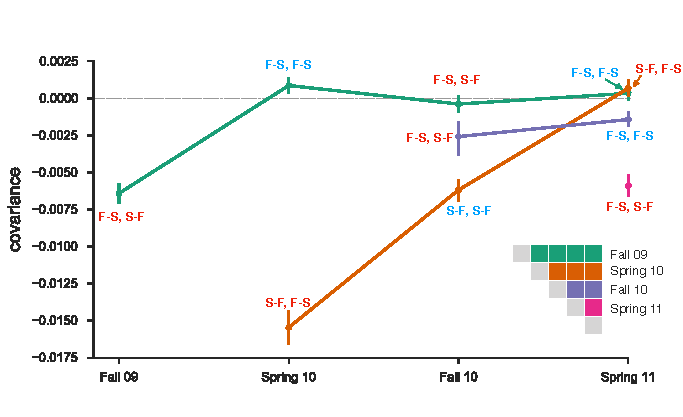
\includegraphics[]{figures/bergland-covs-figure.pdf}

  \caption{Temporal covariances from the \textcite{Bergland2014-ij} study, from
    varying reference generations (e.g. rows along the temporal covariance
    matrix). Each covariance is labeled indicating whether the covariance is
    between two like seasonal transitions (e.g. the covariance between allele
    frequency changes from fall to spring in one year, and fall to spring in
    another) or two dislike seasons (e.g. the covariance between fall to spring
    in one year, and spring to fall in another year). Covariances between like
    transitions are expected to be positive when there is a genome-wide effect
    of fluctuating selection (and these labels are colored blue), while
    covariances between dislike transitions are expected to be negative (and
    these labels are colored red). 95\% confidence intervals were constructed
    by a block-bootstrapping procedure where the blocks are megabase tiles.}

  \label{suppfig:bergland-covs-figure}
\end{figure}

We wanted to establish that our temporal-covariance matrix bias correction was
working correctly. We find that it corrects the relationship between depth and
both variance and covariance (Supplementary Figure
\ref{suppfig:bergland-correction}) as expected.

\begin{figure}[!ht]
  \centering
  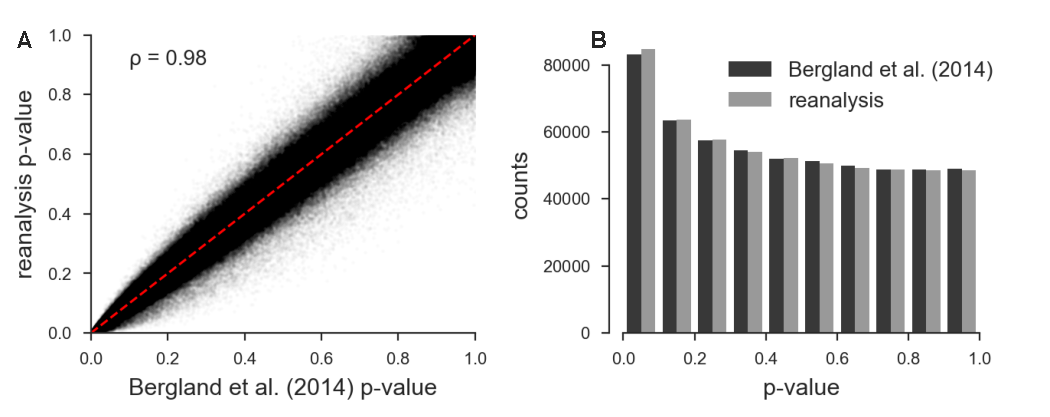
\includegraphics[width=\textwidth]{figures/bergland_pvalues.pdf}

  \caption{\textbf{A}: Scatterplot of the original unadjusted p-values from
    \textcite{Bergland2014-ij} and the p-values from our reanalysis of the same
    data using the same statistical methods; the minor discrepancy is likely
    due to software version differences. \textbf{B}: The histograms of the
    p-values of our reanalysis and the original \textcite{Bergland2014-ij}
    data; again the minor discrepancy is likely due to software differences.
    Overall, our implementation of Bergland et al.'s statistical methods
    produces results very close to the original analysis.}

  \label{suppfig:bergland-pvalue-comparison}
\end{figure}


It is unclear how strong the fluctuations would have to be to generate a
genome-wide average signal of fluctuating selection from temporal covariances.
For example, many loci could still show a signal of fluctuating selection, but
the average signal could be overwhelmed by other signals of other selection. To
investigate whether there was a genome-wide excess of loci showing evidence of
fluctuating selection we reanalyzed the data of \parencite{Bergland2014-ij}
using the same seasonal fluctuating model as the original paper. This model is
a Binomial logit-linked GLM fit per-locus, where the frequencies are regressed
on the Spring/Fall seasons are encoded as a dummy variable. We use the same
binomial weighting procedure as \textcite{Bergland2014-ij}, where the weights
are determined by the effective number of chromosomes, $N_{eff} = (2 n_t d_t -
1) / (2 n_t + d_t)$ ($n_t$ and $d_t$ are the number of diploid individuals and
the read depth at timepoint $t$, respectively). We fit this model on all loci
marked as used in the VCF provided with the \textcite{Bergland2014-ij} study
(doi:10.5061/dryad.v883p). Overall, our p-values for the Wald test for each
locus closely match those of the original paper (Pearson correlation
coefficient 0.98, p-value < $2.2 \times 10^{-16}$; see Supplementary Figure
\ref{suppfig:bergland-pvalue-comparison} A), and the histograms of the p-values
are nearly identical (Supplementary Figure
\ref{suppfig:bergland-pvalue-comparison} B). \textcite{Bergland2014-ij} find
loci with a significant association with season after a Benjamini and Hochberg
FDR p-value adjustment \parencite{Benjamini1995-jy}, however, the null
hypothesis of the Wald test does not give us an idea of the expected number of
variants that may spuriously fit the pattern of seasonal fluctuating selection
as it does not account for genetic drift or other forms of hitchhiking.

\begin{figure}[!ht]
  \centering
  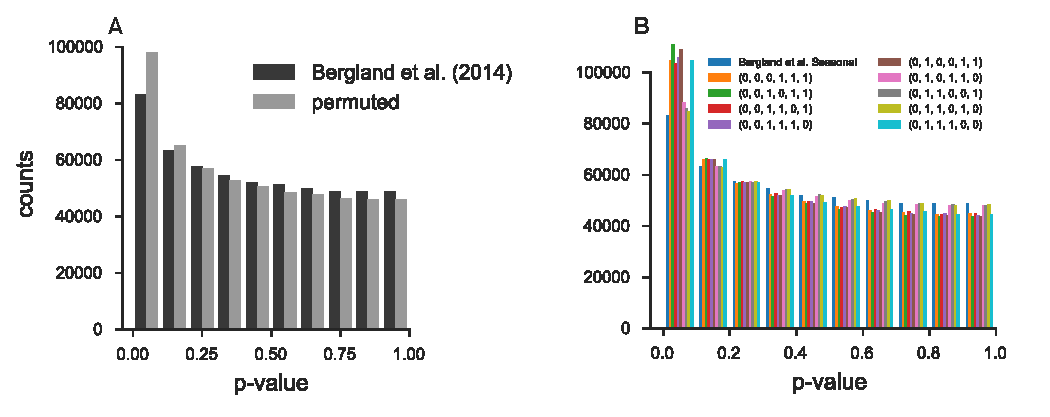
\includegraphics[width=\textwidth]{figures/bergland-combined-hists.pdf}

  \caption{\textbf{A}: Histogram of original \textcite{Bergland2014-ij}
    seasonal p-values and p-values creating by randomly permuting the seasons
    at each locus. \textbf{B}: Histogram of original \textcite{Bergland2014-ij}
    p-values alongside all unique permutations (ignoring symmetries that lead
    to identical p-values).}

  \label{suppfig:bergland-pvalue-hist}
\end{figure}


\begin{figure}[!ht]
  \centering
  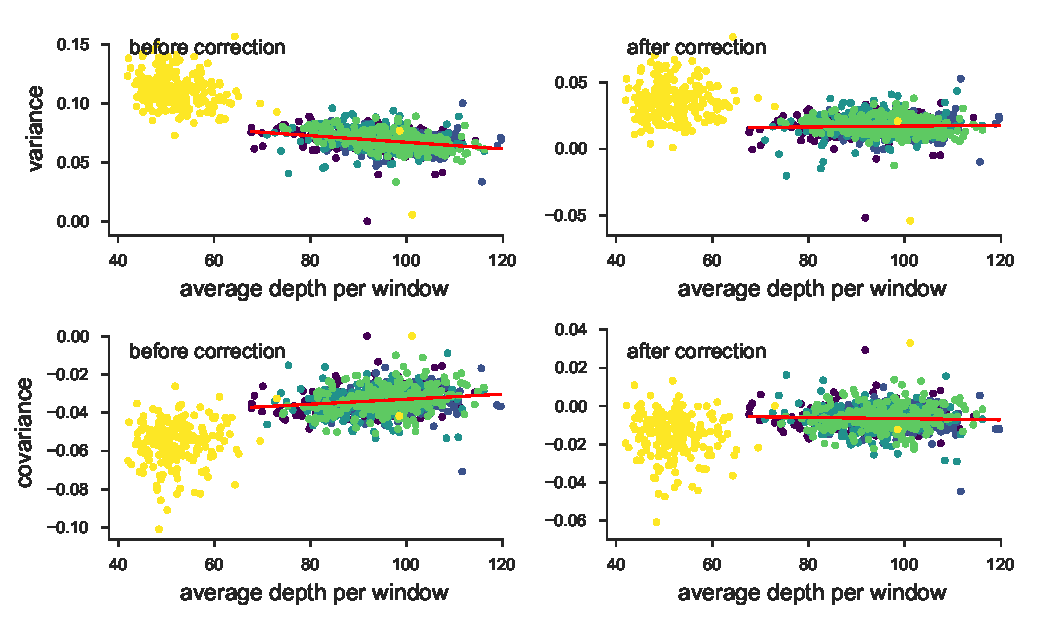
\includegraphics[width=\textwidth]{figures/bergland-correction-plot.pdf}

  \caption{The variance and covariances from the \textcite{Bergland2014-ij}
    study, calculated in 100kb genomic windows plotted against average depth in
    a window before and after bias correction. Each panel has a least-squares
    estimate between the variance and covariance, and the average depth.
    The bias correction procedure is correcting sampling bias in both the variance
    and covariance such that the relationship with depth is constant. Colors
    indicate the different chromosomes of \emph{D. melanogaster}; we have
    excluded the X chromosome (yellow points; chromosome 4 was not in the
    original study) from the regression due to large differences in average
    coverage.}

  \label{suppfig:bergland-correction}
\end{figure}



To investigate whether there is a genome-wide evidence of an enrichment of
fluctuating selection we created an empirical null distribution by randomly
permuting the season labels and re-running the per-locus seasonal GLM model, as
proposed by \textcite{Machado2018-cs}. We find, regardless of whether we
permute at the locus-level or the permutation replicate-level, that the
observed seasonal p-value distribution \textcite{Bergland2014-ij} is not
enriched for significant p-values beyond what we would expect from the
permutation null. In fact, there appears there is more enrichment for low
p-values when seasonal labels are randomly permuted (Supplementary Figure
\ref{suppfig:bergland-pvalue-hist}, suggesting by random chance we might expect
more variants with a seasonal fluctuating pattern than found in the original
\textcite{Bergland2014-ij} study. While surprising, this could be explained by
the presence of temporal structure across the samples not consistent with
seasonal fluctuating selection. Some fraction of the permutations happen to fit
this structure well, leading to an enrichment of small p-values. This
non-seasonal temporal structure is also evident in our temporal covariances
(Supplementary Figure \ref{suppfig:bergland-covs-figure}), where we see strong
evidence of selection (non-zero temporal covariances), yet the pattern does not
follow that of seasonal fluctuating selection.  


\subsection{Simulation Results}

We conducted extensive simulations to understand how temporal covariance,
$G(t)$, and convergence correlations behave under (1) different quantitative
genetic fitness models, (2) different trait architectures (e.g. varying levels
of $V_A$ for fitness and the number of sites affecting fitness) and (3)
background selection. Furthermore, we use two population simulations to
investigate how convergence correlations depend on (1) the population sizes of
each selection line sampled from the main population, and (2) the direction the
trait is selected on in each line (i.e. in the same direction, differing
directions, or only one lines elected).

Due to the high computational burden of forward simulations, we modeled a
single 50 megabase region in a population of $N = 1000$ diploid individuals
with a neutral variant mutation rate of $10^{-8}$ and a recombination rate of
$10^{-8}$ per basepair. This is roughly analogous to a XXX chromosome of
\emph{Drosophila melanogaster}; however with this small population size and
mutation rate, the population mutation rate $\theta$ for the entire region
leads to far fewer neutral sites to calculate covariances and other statistics
on than expected for a region this length in \emph{D.  melanogaster}. Since our
main goal is to understand how the dynamics of statistics used in the paper and
how they are affected by background selection, fitness model, and trait
architecture, we use population frequencies rather than sampling frequencies.

All forward simulations were conducted using SLiM \parencite{Haller2019-vu},
and the simulation routines are available in the Github repository
\url{https://github.com/vsbuffalo/cvtk/}.

\subsubsection{The Effects of the Genetic Architecture}
\label{supp:genetic-arch}

We first investigated the effects of the selected trait's genetic architecture
on temporal covariances and $G(t)$ by neutrally burning in a population for
$10N$ generations, and selecting on the trait with an exponential fitness
function. By using an exponential fitness function (a form of selection
multiplicative across sites), we ensure there is no build up of LD due to
selection (XXX) and epistasis; this serves as the simplest directional
selection model of a trait to understand the effects of genetic architecture on
the statistics we have used in the paper.

During this burnin, sites were either marked as neutral (with mutation rate
$\mu_\mathrm{neutral} = 10^8$ per gamete per generation) or contributed to the
trait's value (with mutation rate $\mu_\mathrm{trait}$), but were not selected
on until generation $10N + 5$ (the five generations after burnin serve as a
neutral control). The trait mutation rate, $\mu_\mathrm{trait}$ was set by
targeting a particular architecture, the number of selected sites, $L$. Each
site contributing to the trait's value was randomly chosen to have effect size
$\pm \alpha$ with equal probability, where $\alpha$ was set to target a
particular additive genetic variance for the trait, $V_A$, for the target
number of selected sites $L$. 

Overall, we confirm a finding in \parencite{Buffalo2019-io} that the initial
expected temporal covariance conditioned on $V_A$, is invariant to the number
of loci determining the trait's value, $L$ (Supplementary Figure
\ref{suppfig:sim-expfit-covs}). We do find some evidence that the decay in
temporal covariance is faster when the trait has a monogenic basis (see the
third column of Supplementary Figure \ref{suppfig:sim-expfit-covs}); this is
expected the selection coefficients are larger for these monogenic simulations,
leading to faster allele frequency changes and a rapid change in additive
genetic variance. 

In our previous work, we did not investigate the affect of trait architecture
on our measure $G(t)$.  Using the exponential fitness function simulations, we
also calculated $G(t)$ for each of the replicate simulations. We find that
across replicates, the $G(t)$ trajectories can vary considerably depending on
the number of sites ($L$) determining the trait's value (Supplementary Figure
\ref{suppfig:sim-expfit-Gs}). When a trait is monogenic ($L \approx 1$), $G(t)$
trajectories vary considerably across replicate lines, as certain lines may not
contain the few selected alleles (top row of Supplementary Figure
\ref{suppfig:sim-expfit-Gs}). However, with a polygenic trait, ($L \ge 100$),
the $G(t)$ trajectories across replicates are all quite close as each replicate
contains an abundance of alleles that affect the trait's value (bottom rows of
Supplementary Figure \ref{suppfig:sim-expfit-Gs}). Comparing the simulated
$G(t)$ replicate trajectories of Supplementary Figure
\ref{suppfig:sim-expfit-Gs} with the \textcite{Barghi2019-qy} $G(t)$
trajectories in Figure \ref{fig:figure-1}B, we again confirm a finding of
\textcite{Barghi2019-qy}: that there is considerable genetic redundancy among
beneficial alleles. We should note that our simplified simulation routines are
slightly different from the \textcite{Barghi2019-qy} study in that the burnin
populations are all independent; however we expect the same qualitative result. 

\vb{TODO: note about different burnin pops?}


\begin{figure}[!ht]
  \centering
  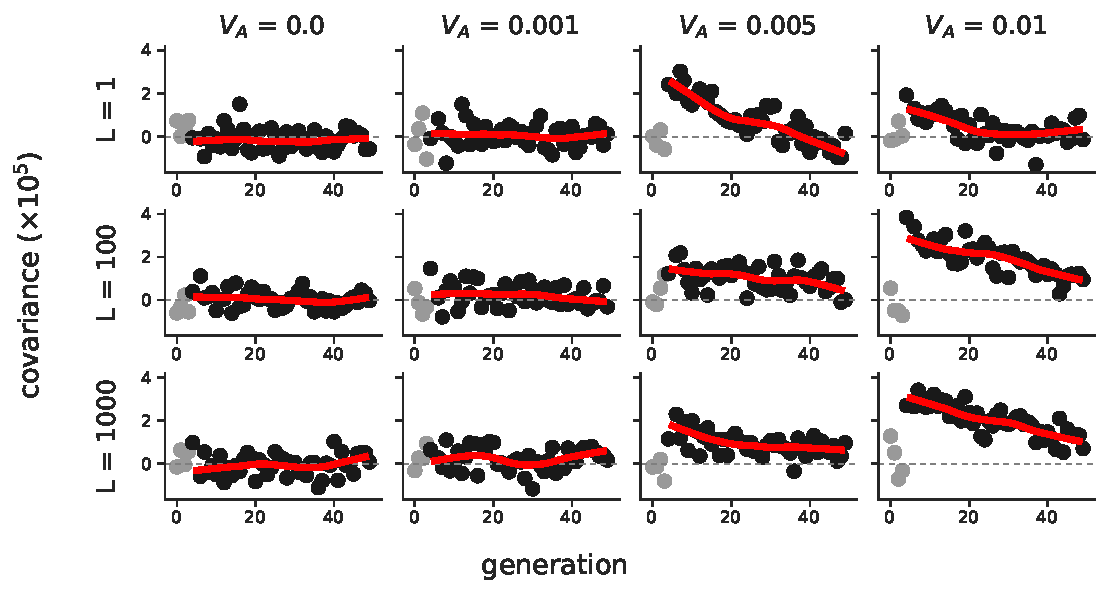
\includegraphics[width=\textwidth]{figures/fig-architecture-cov.pdf}

  \caption{The temporal covariances $\cov(\Delta p_5, \Delta p_t)$ from the
    onset of selection (generation 5) to a later time point $t$, which varies
    along the x-axis, across a variety of different trait additive genetic
    variances ($V_A$, columns) and number of sites contributing to the trait
    ($L$, rows). Each point is the temporal covariance averaged over 50
    replicate simulations; dark gray points are temporal covariances after the
    onset of selection, and light gray points are before. The red line is a
    loess smoothed curve through the covariances after the onset of selection.
    Selection on the trait was imposed through an exponential fitness function.}

  \label{suppfig:sim-expfit-covs}
\end{figure}


\begin{figure}[!ht]
  \centering
  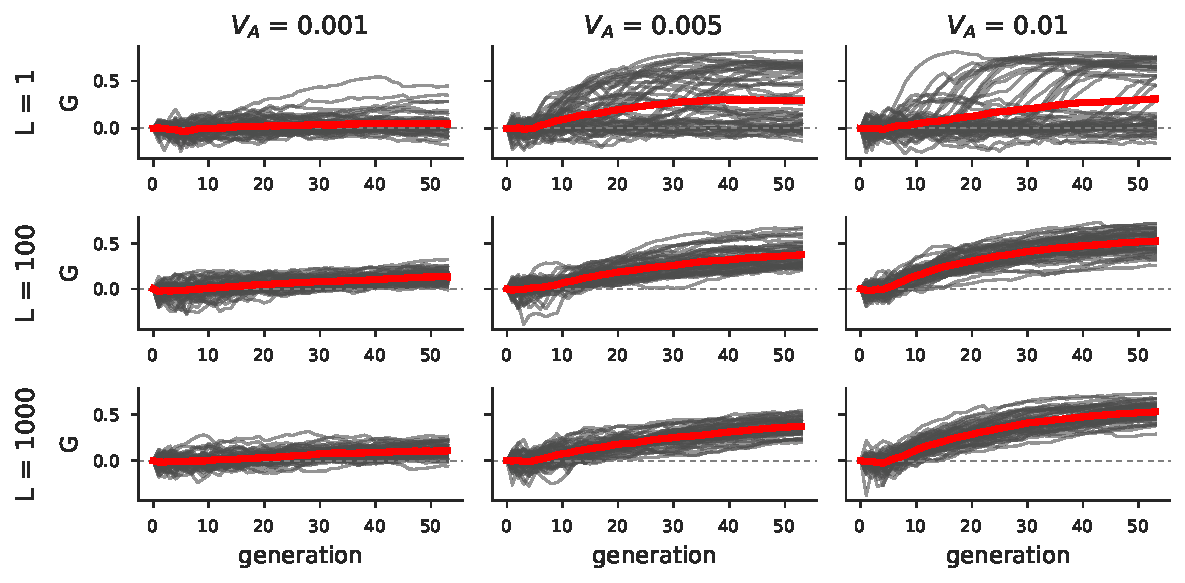
\includegraphics[width=\textwidth]{figures/fig-architecture-G.pdf}

  \caption{The $G(t)$ trajectories of 50 replicate simulations, across
    different trait architectures ($L$ is the target number of sites affecting
    the trait's value, and $V_A$ is the target trait additive genetic
    variance).  The red line is the mean trajectory across all replicate
  simulations. Like Supplementary Figure \ref{suppfig:sim-expfit-covs}, the
onset of selection is five generations after the $10N$ generation burnin; this
is evident by the initial flat section of the $G(t)$ trajectory.}

  \label{suppfig:sim-expfit-Gs}
\end{figure}

\subsubsection{Sampling in Temporal Blocks}

In our analysis of the \textcite{Barghi2019-qy} data, we describe our statistic
$G(t)$ as an lower bound for two reasons: (1) the population is sequenced every
ten generations, meaning the temporal covariances between adjacent generations
cannot contribute to the numerator of $G(t)$ but contribute to the denominator,
and (2) the estimate of $G(t)$ ignores linked selection's contribution to the
variance in allele frequency change (this is the difference between $G$ and
$G'$, the latter of which includes these variance terms \cite{Buffalo2019-io}).
To verify that $G(t)$ estimated every ten generations is indeed a lower bound,
we used a simulation procedure similar to the exponential fitness function
simulations (described in Supplementary Material Section
\ref{supp:genetic-arch}), and calculated the temporal covariances and $G(t)$
both each generation, and every ten generations. Unlike the simulations
described in \ref{supp:genetic-arch}, we began selection at $10N$ generations,
and used trait $V_A = 0.01$ and $L = 1000$ sites affecting the trait. 

First, comparing $G(t)$ when sampling population frequencies every generation
versus every ten generations, we confirm that the ten-generation block $G(t)$
is a lower bound of the true every generation $G(t)$ (red and blue lines in
Supplementary Figure \ref{suppfig:supp-blocks}A). Furthermore, since we control
the population size in our simulations at $N = 1000$ diploids, we know the
drift effective population size in the absence of selection. This allows us to
estimate $G(t)'$, which is a measure of $G(t)$ that accounts for the linked
selection's inflation of the variance in allele frequency change between two
generations (equation 26, \cite{Buffalo2019-io}). Plugging in the drift
effective population size $N_e = 1000$ into the expression for $G'(t)$ and
using the $\var(p_t - p_0)$ calculated for different $t$'s, we see that the
every generation $G(t)$ that does not account for linked selection's inflation
of $\var(\Delta p_t)$ does underestimate the true impact of linked selection as
expected (dashed gray line in Supplementary Figure \ref{suppfig:supp-blocks}A).

To further understand the effects of calculating temporal covariances every ten
generations rather than every generation, we also compared their magnitudes and
decay rates using the simulations described above. We find that ten generation
block temporal covariances are orders of magnitude larger but decay at similar
rates (see Supplementary Figure \ref{suppfig:supp-blocks}B; note the two y-axis
scales are different). The larger magnitude is expected, as each ten generation
block temporal covariance is the sum of XXX.


\begin{figure}[!ht]
  \centering
  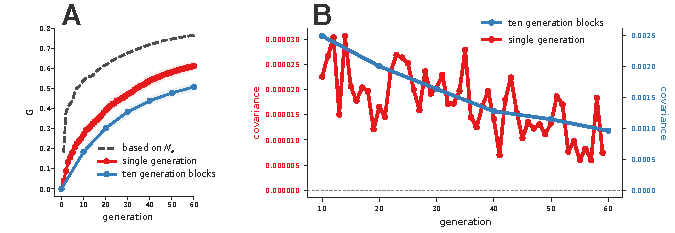
\includegraphics[width=\textwidth]{figures/fig-supp-blocks.pdf}

  \caption{A: The $G(t)$ averaged over 50 replicate simulations with $V_A =
    0.01$ and $L = 1000$. The blue line shows $G(t)$ calculated over ten
    generation blocks, similar to the calculation of temporal covariances of
    the \textcite{Barghi2019-qy} study. The red line shows the average $G(t)$
    estimates when the population is sampled every generation and all
    covariances can contribute to the numerator of $G(t)$. The dashed gray line
    indicates the $G(t)'$ estimate, which uses the known drift effective
    population size of the simulations. B: The temporal covariances calculated
    each generation (red line) and on ten generation blocks (blue line) using the
    same simulation data.}

  \label{suppfig:supp-blocks}
\end{figure}

\subsubsection{Convergence Correlations}

\begin{figure}[!ht]
  \centering
  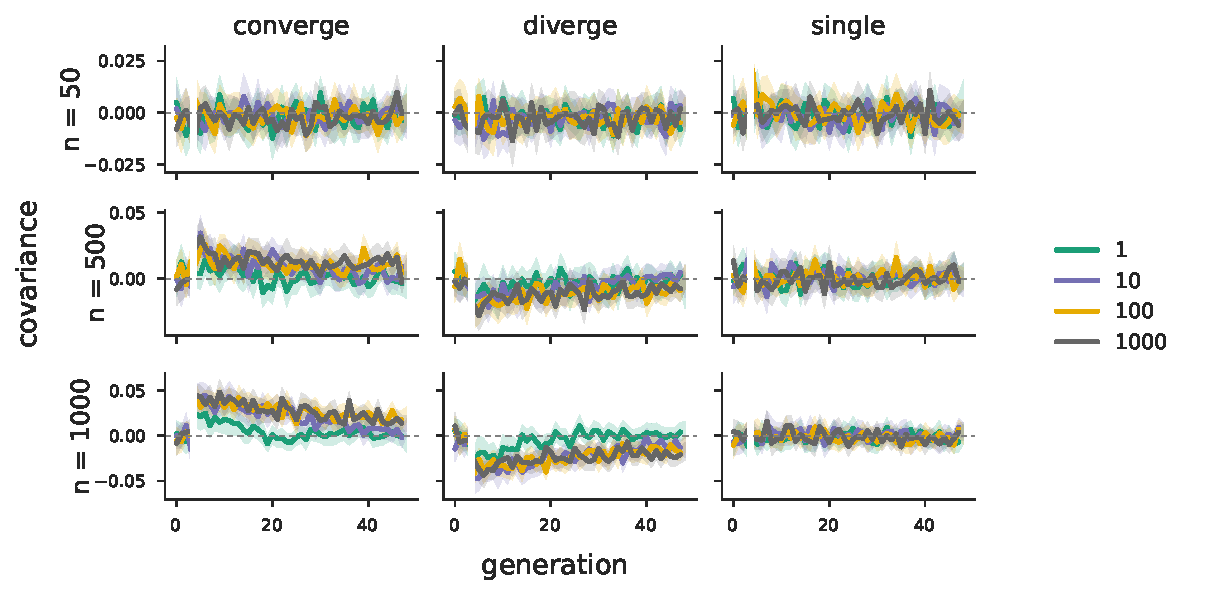
\includegraphics[width=\textwidth]{figures/fig-convergence-corrs.pdf}

  \caption{}

  \label{suppfig:supp-blocks}
\end{figure}


\subsubsection{Background Selection's Effect on Temporal Covariance}




\begin{figure}[!ht]
  \centering
  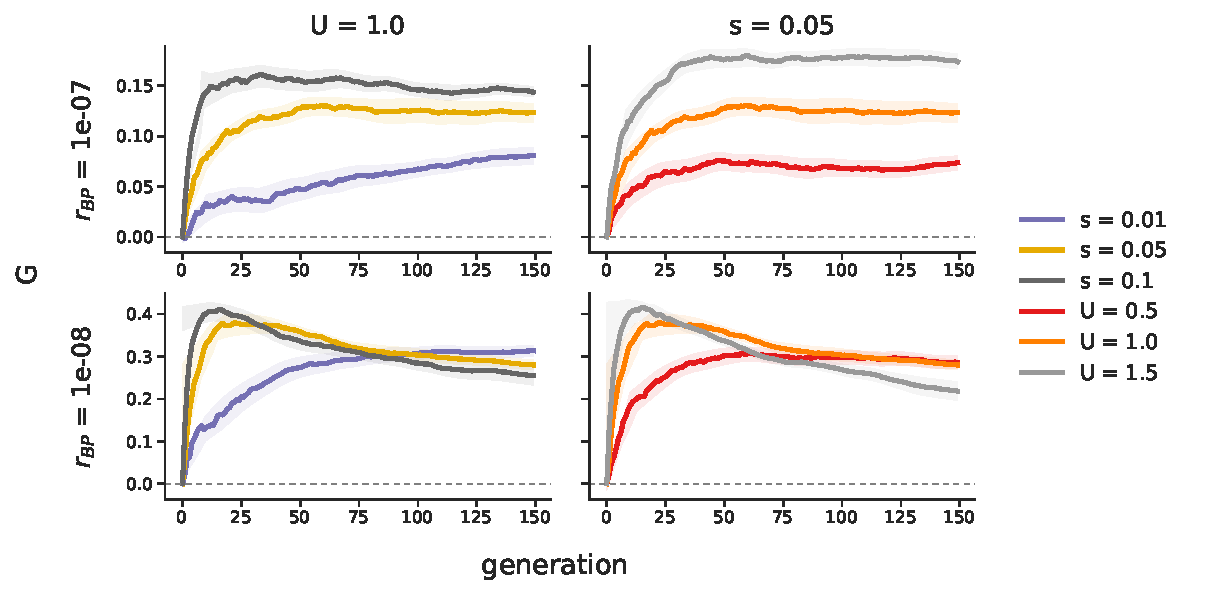
\includegraphics[width=\textwidth]{figures/fig-bgs-G-without-fixations.pdf}

  \caption{}

  \label{suppfig:supp-bgs-g}
\end{figure}


\begin{figure}[!ht]
  \centering
  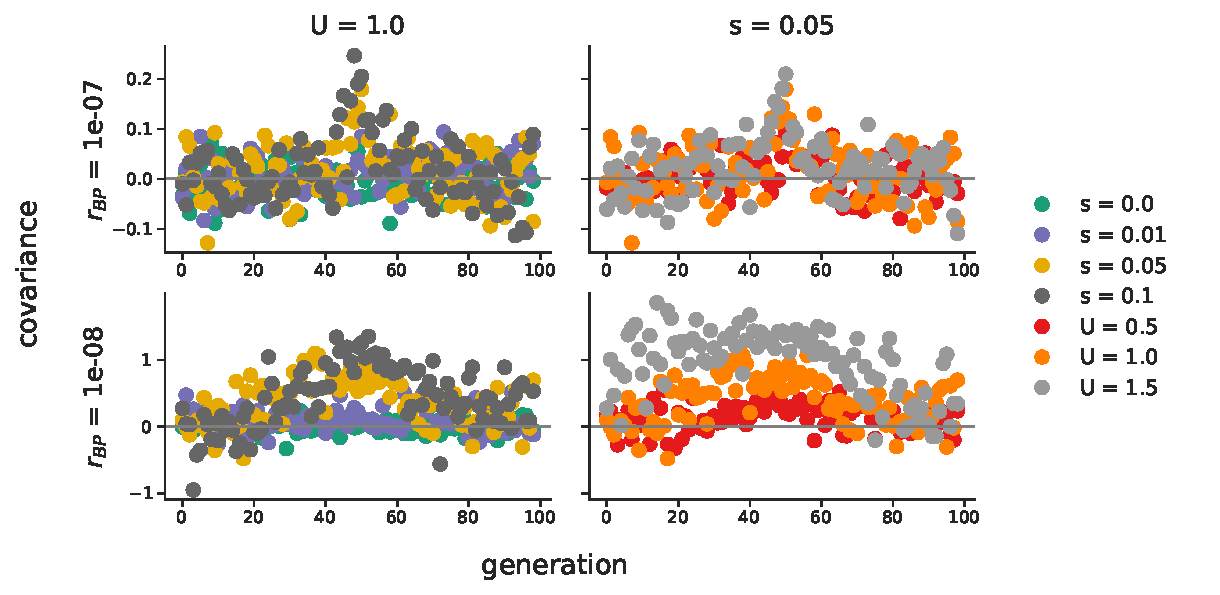
\includegraphics[width=\textwidth]{figures/fig-bgs-covars-without-fixations.pdf}

  \caption{}

  \label{suppfig:supp-bgs-covs}
\end{figure}




\subsubsection{The Effect of Fixations}

In analyzing both the empirical datasets included in our study and our
simulation results, we noticed the temporal covariances and $G(t)$ statistics
are sensitive to how fixations (i.e. when a site is polymorphic but is fixed or
lost during the course of its trajectory) are handled. Through simulations and
comparing the results of analyzing our empirical datasets both ways, we have
found trade-offs to both approaches, but overall find that not removing fixed
sites is a more conservative, safer approach, and is what we use throughout our
paper. 

\begin{figure}[!ht]
  \centering
  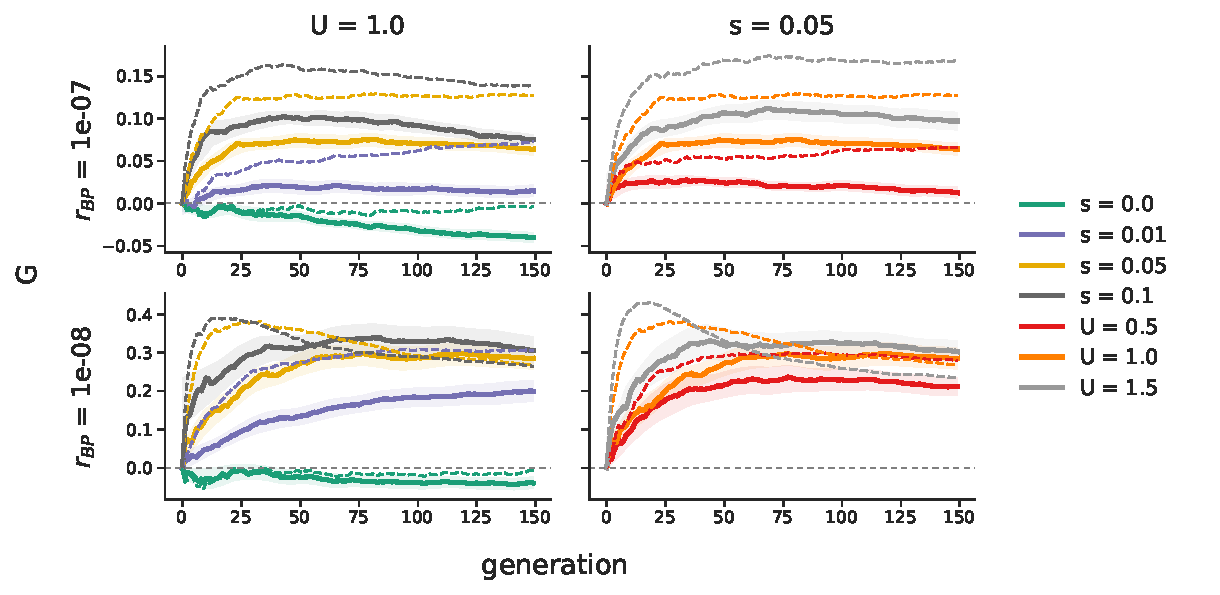
\includegraphics[width=\textwidth]{figures/fig-bgs-G-with-fixations.pdf}

  \caption{$G(t)$ trajectories from background selection simulations both
  including fixed sites (solid lines) and not including fixed sites (dashed
lines). The dashed lines are identical to those in Supplementary Materials
Figure \ref{suppfig:supp-bgs-g}. As expected, including fixed sites shrinks the
$G(t)$ towards zero, and in some cases, they can become negative.}

  \label{suppfig:supp-bgs-g-fix}
\end{figure}



Temporal covariances (and related statistics like convergence correlations,
$G(t)$, etc.) are calculated on allele frequency changes, $\Delta p_t$; when an
allele is fixed or lost, the allele frequency changes are zero thereafter
$\Delta p_t = 0$. When temporal covariance is calculated by averaging over the
loci in a region or across the genome, fixed sites zero out the terms in the
sum of the right hand side of temporal covariance, $\cov(\Delta p_t, \Delta
p_s) = \E(\Delta p_t \Delta p_s) - \E(\Delta p_t) \E(\Delta p_s)$ and can
shrink the second terms towards zero. From simulations using population
frequencies (e.g. no sampling noise), we have found that including neutral
sites into the temporal covariance calculation that are lost or fix will tend
to shrink the covariance towards zero, and in some cases create spurious
negative temporal covariances. We observed this when conducting the background
selection simulations of Supplementary Materials Section XXX, and have included
an alternative version of this figure that includes $G(t)$ trajectories
calculated by including fixed neutral sites (Supplementary Figure
\ref{suppfig:supp-bgs-g-fix}). We find, as expected, $G(t)$ trajectories
calculated including fixed sites are shrunk towards zero, and in some cases,
can become negative. In contrast, the $G(t)$ trajectories ignoring fixations
(dashed lines in Supplementary Figure \ref{suppfig:supp-bgs-g-fix}) are higher.

XXX truncation selection, exponential.


While simulation results using population frequencies show that including fixed
sites has the downside of shrinking the temporal covariance towards zero, and
in some cases can create negative covariances, we have found excluding fixed
sites on sample frequency data has a severe drawback: low frequency alleles
will occasionally not be observed at a sample timepoint (leading to a frequency
of zero of the minor allele), and excluding these observations (instead of
treating it as a trajectory that has a 0 frequency timepoint) biases estimates.
We observed this bias created by ignoring fixed or loss sites by comparing our
$N_e$ estimates for the \textcite{Barghi2019-qy} study (estimated from the
total variance in allele frequency change) with the estimates from the original
paper. We found that ignoring fixed or lost sites (by treating them as missing
data in calculating the covariances) led to many low-frequency alleles not
contributing to the variance, leading this statistic to be calculated on more
intermediate frequency alleles and thus biasing the $N_e$ estimate downwards.
Additionally, we tried only dropping fixed or loss sites from the temporal
covariance calculations that were at the end or the beginning of a trajectory
(e.g., as if the site was created by a new mutation or fixed); while this
ameliorated some of this bias, it still did not lead to $N_e$ estimates
congruent with the original studies. Overall, we found by trying all these
approaches that not removing fixed or lost sites was the best way to deal with
sample allele frequencies that could be missing from some timepoints. 

Still, we wanted to ensure that our empirical re-analyses were robust to our
choice of how we handled fixed sites. Given that under some simulation
conditions, we find that spurious negative covariances can occur when fixations
are included, we wanted to ensure that our result that the temporal covariances
of \textcite{Barghi2019-qy} that become negative at later timepoints are not an
artifact of the way fixations are handled. First, we regenerated Figure 1 A and
B, except with temporal covariances and $G(t)$ calculated excluding fixed or
lost sites. We find the same qualitative results regardless of whether we
include or exclude fixed/lost sites; importantly, we still see a significant
signal that the temporal covariances at later timepoints become negative. As
expected the temporal covariances are lessened by excluding fixed sites. 

XXX


\begin{figure}[!ht]
  \centering
  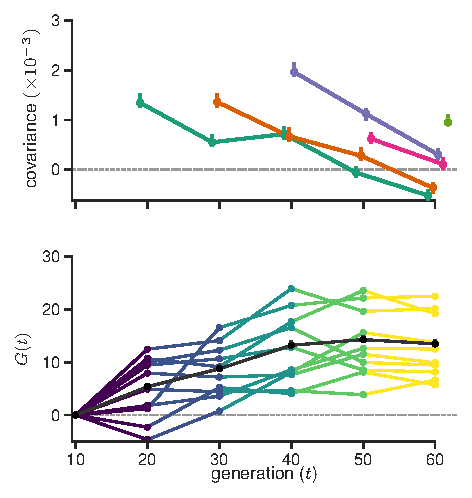
\includegraphics[width=0.6\textwidth]{figures/figure-1-G-covs-nofix.pdf}

  \caption{A version of Figure 1 A and B where sample frequencies of zero or
    one are ignored, e.g. due to fixation, are ignored. Like the original
    Figure 1 in the main text, the 95\% pivot confidence intervals are via a
    bootstrapping procedure; note that we find excluding fixed sites leads to
  more asymmetric confidence intervals. Overall, we find that despite handling
fixed/lost sites differently, we still find significant negative temporal
covariances at later timepoints.}

  \label{suppfig:supp-fig-1-nofix}
\end{figure}



\setcounter{section}{1}
\section*{Supplementary Figures}

\subsection{PCA of \textcite{Barghi2019-qy} replicates}

\begin{figure}[!ht]
  \centering

  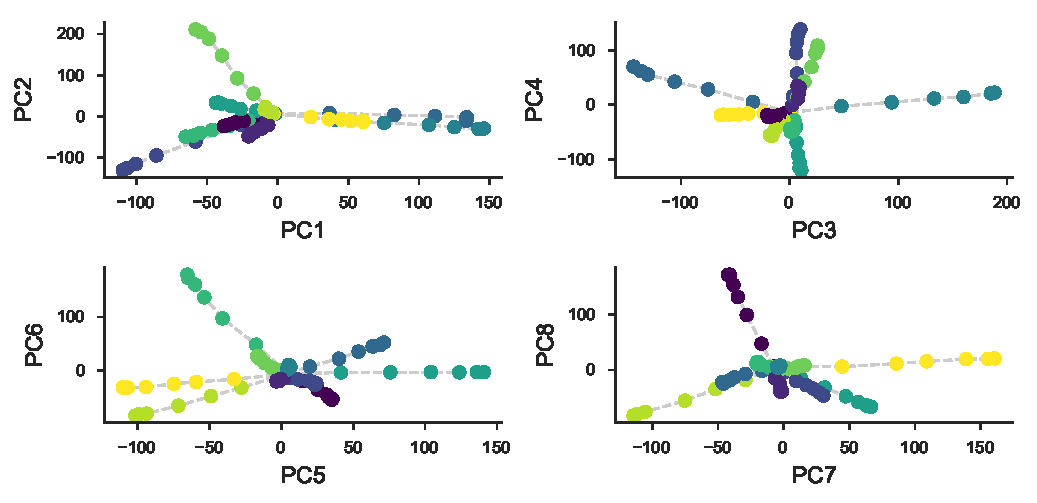
\includegraphics[]{figures/barghi-panel-pca.pdf}

  \caption{A PCA on the centered and standardized population frequencies for
  each replicate (each color) for all its sequenced timepoints (the connected
  series of points). All replicates start from the same source population, and
  thus are overlapping in the center; as each replicate evolves independently it
  diverges from the other replicates in PCA space.}
  
  \label{suppfig:barghi-pca}
\end{figure}

\subsection{Bias Correction for \textcite{Barghi2019-qy}}

We have investigated the effectiveness of our correction on real data by
exploiting the relationship between sampling depth and the magnitude of the
variance and covariance biases, and comparing the observed variances and
covariances before and after correction. We plot the variance and covariance
(between adjacent timepoints) before and after the bias correction against the
average sample depth in 100kb genomic windows in Figure
\ref{suppfig:barghi-correction}. Overall, we find the biased-correction
procedure removes the relationship between variance and covariance and depth, indicating it is working adequately.

\begin{figure}[!ht]
  \centering
  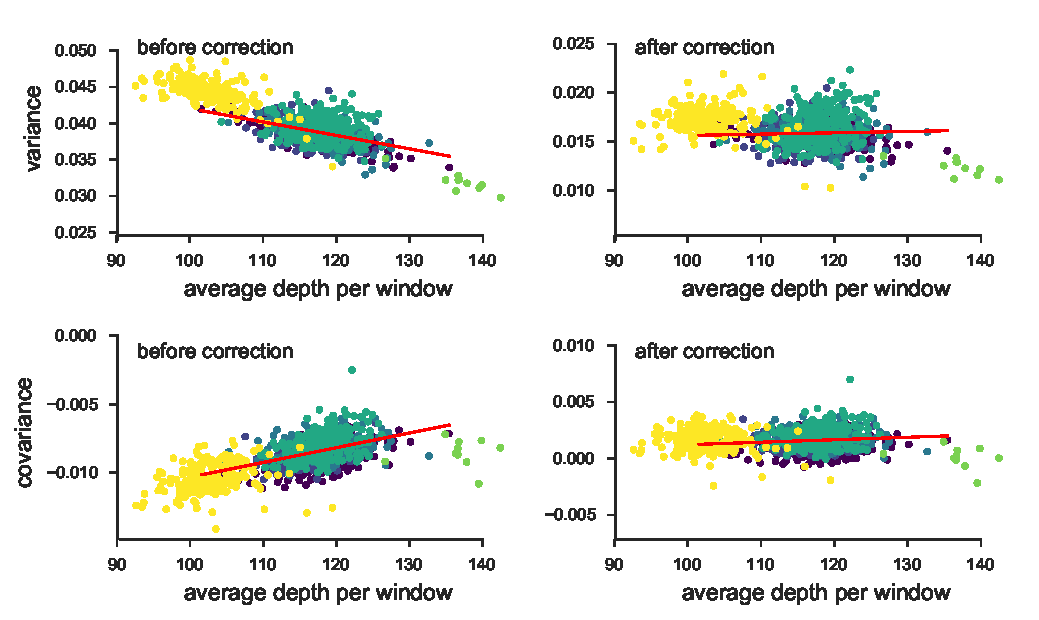
\includegraphics[]{figures/barghi-correction-plot.pdf}

  \caption{The variance and covariances from the \textcite{Barghi2019-qy}
    study, calculated in 100kb genomic windows plotted against average depth in
    a window before and after bias correction.  Each panel has a least-squares
    estimate between the variance and covariance, and the average depth.
    Overall, the bias correction corrects sampling bias in both the variance
    and covariance such that the relationship with depth is constant. Colors
    indicate the different chromosomes of \emph{D. simulans}; we have excluded
  the X chromosome (yellow points) and chromosome 4 points (green points to far
right) from the regression due to large differences in average coverage.}

  \label{suppfig:barghi-correction}
\end{figure}

\clearpage

\subsubsection{\textcite{Barghi2019-qy} Temporal Covariances Per Replicate}
\begin{figure}[!ht]
  \centering
  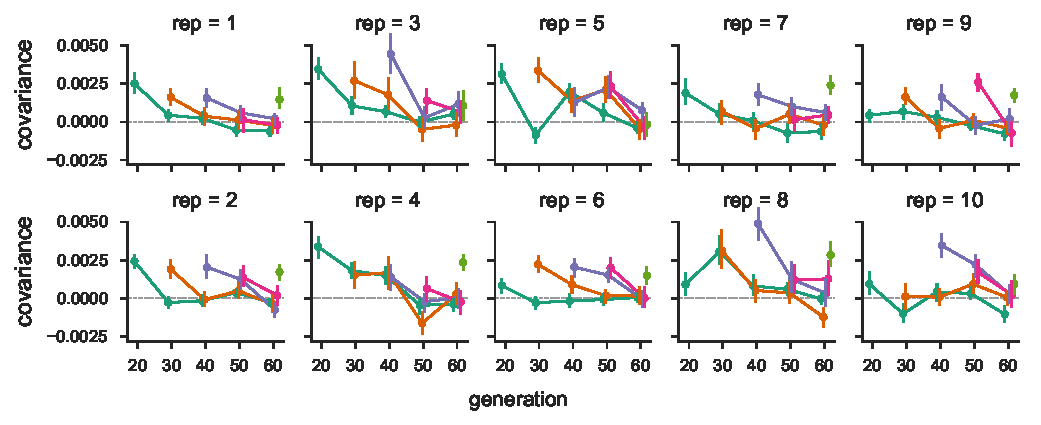
\includegraphics[width=\textwidth]{figures/barghi-cov-panels.pdf}

  \caption{The temporal covariances from the \textcite{Barghi2019-qy} study,
  for each replicate individually. As in Figure \ref{fig:figure-1}, each line
  follows the temporal covariances from some initial reference generation through
  time, which represent the rows of temporal covariance matrix.}

  \label{suppfig:barghi-cov-panels}
\end{figure}


\clearpage

\subsection{\textcite{Barghi2019-qy} Trimmed Window Covariances}
\begin{table}
  \centering
  \footnotesize
  \centering
  \begin{tabular}{l c c c c c c}

    s & t & median & median 95\% CI & trimmed mean & trimmed mean 95\% CI \\ \hline
    0 & 10 & 1.629 & $[1.532, 1.738]$ & 1.874 & $[1.777, 1.969]$ \\
    0 & 20 & 0.371 & $[0.276, 0.465]$ & 0.491 & $[0.403, 0.585]$ \\
    0 & 30 & 0.479 & $[0.4, 0.589]$ & 0.516 & $[0.434, 0.602]$ \\
    0 & 40 & 0.059 & $[-0.012, 0.15]$ & 0.027 & $[-0.05, 0.099]$ \\
    0 & 50 & -0.204 & $[-0.271, -0.125]$ & -0.259 & $[-0.329, -0.187]$ \\
    10 & 20 & 1.549 & $[1.427, 1.659]$ & 1.722 & $[1.617, 1.83]$ \\
    10 & 30 & 0.438 & $[0.339, 0.539]$ & 0.506 & $[0.399, 0.609]$ \\
    10 & 40 & 0.233 & $[0.149, 0.328]$ & 0.254 & $[0.159, 0.343]$ \\
    10 & 50 & -0.355 & $[-0.454, -0.289]$ & -0.319 & $[-0.401, -0.237]$ \\
    20 & 30 & 1.981 & $[1.856, 2.095]$ & 2.195 & $[2.084, 2.302]$ \\
    20 & 40 & 0.792 & $[0.698, 0.894]$ & 0.903 & $[0.815, 0.999]$ \\
    20 & 50 & 0.123 & $[0.042, 0.207]$ & 0.221 & $[0.141, 0.309]$ \\
    30 & 40 & 1.296 & $[1.208, 1.425]$ & 1.385 & $[1.287, 1.483]$ \\
    30 & 50 & 0.07 & $[-0.037, 0.183]$ & 0.116 & $[0.023, 0.21]$ \\
    40 & 50 & 1.36 & $[1.271, 1.446]$ & 1.513 & $[1.427, 1.601]$ \\


   \end{tabular}
   \caption{Table of median of windowed covariance estimates ($\cov(\Delta p_s,
     \Delta p_t) \times 100$) between generations $t$ and $s$ and the trimmed
     mean windowed covariance which excludes the lower and upper 5\% windows
     with the highest covariance.}
  \label{supp:table-trimmed-mean}

\end{table}



Here we report median and trimmed mean of the windowed covariances
(Supplementary Table \ref{supp:table-trimmed-mean}). We note that the median
covariance is also limiting result of a trimmed mean that symmetrically
excludes the upper and lower $\alpha$ tails to calculate the trimmed average
windowed covariance. As $\alpha$ increases to 0.5, the trimmed covariance
converges to the median windowed covariance (by the definition of the median;
see Supplementary Figure \ref{suppfig:barghi-trimmed-mean}). Thus our genomic
temporal covariances are non-zero due to the impact of selection on many
genomic windows.  


\begin{figure}[!ht]
  \centering
  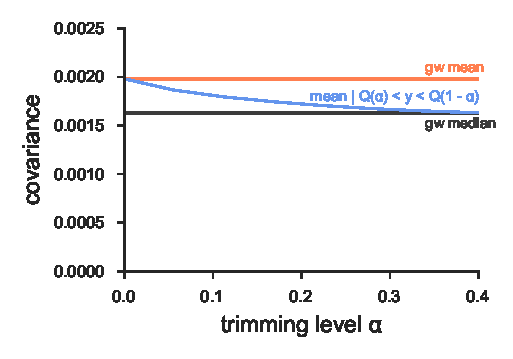
\includegraphics[]{figures/barghi-trimmed-mean.pdf}

  \caption{The genome-wide covariance ($\cov(\Delta p_0, \Delta p_10)$ pooling
    all replicates) averaged (red line) and the median windowed covariance
    (blue) for the \textcite{Barghi2019-qy} dataset. The trimmed average window
    covariance, excluding the $\alpha$ lower and upper tails, converges to the
     median windowed covariance. This indicates that genome-wide covariance are
     not being overly dominated by a large-effect loci in few windows.}

  \label{suppfig:barghi-trimmed-mean}
\end{figure}



\clearpage

\subsection{\textcite{Barghi2019-qy} Empirical Null and Windowed Covariance Distributions}

\begin{figure}[!ht]
  \centering
  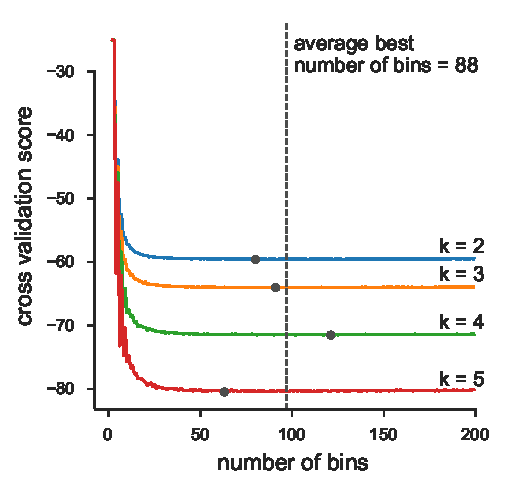
\includegraphics[]{figures/barghi-cross-validation-binsize.pdf}

  \caption{We chose number of bins used in the histograms of Figure
    \ref{fig:figure-3} via an analytic expression for the cross-validation
    risk, based on the equation 6.16 of (\cite{Wasserman2006-jl}, p. 129).
    Above, we plot the cross-validation risk for various numbers of bins, for
    each of the four off-diagonals of the temporal covariance matrix that we
    analyze. Overall, because the number of data points is large, oversmoothing
    is less of a problem, leading the cross-validation risk to be relatively
    flat across a large number of bins. Each gray point indicates the minimal
    risk for a particular off-diagonal, and the dashed line indicates the best
    average binwidth across off-diagonals.}
  \label{suppfig:barghi-cross-validation-binsize}
\end{figure}



\begin{figure}[!ht]
  \centering
  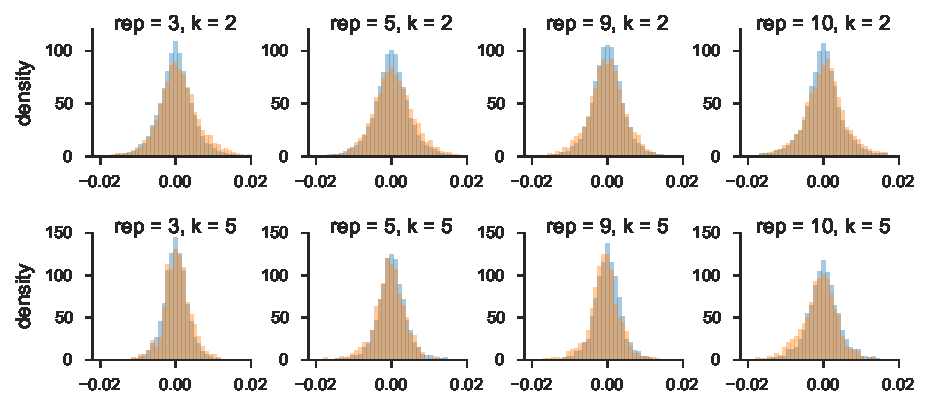
\includegraphics[]{figures/barghi-offset-replicate-panels.pdf}

  \caption{The distribution of windowed temporal covariances alongside the
    empirical neutral null for five randomly sampled replicates (columns), for
    $k=2$ (first row) and $k=5$ (second row). The main figure of the paper
    pools all replicate window and empirical neutral null covariances; we show
    here the windowed temporal covariances tend to shift from being positive (a
    heavier right tail) to become more negative (a heavier left tail) through
    time within particular replicates.}
  
  \label{suppfig:barghi-offset-replicate-panels}
\end{figure}



\begin{figure}[!ht]
  \centering
  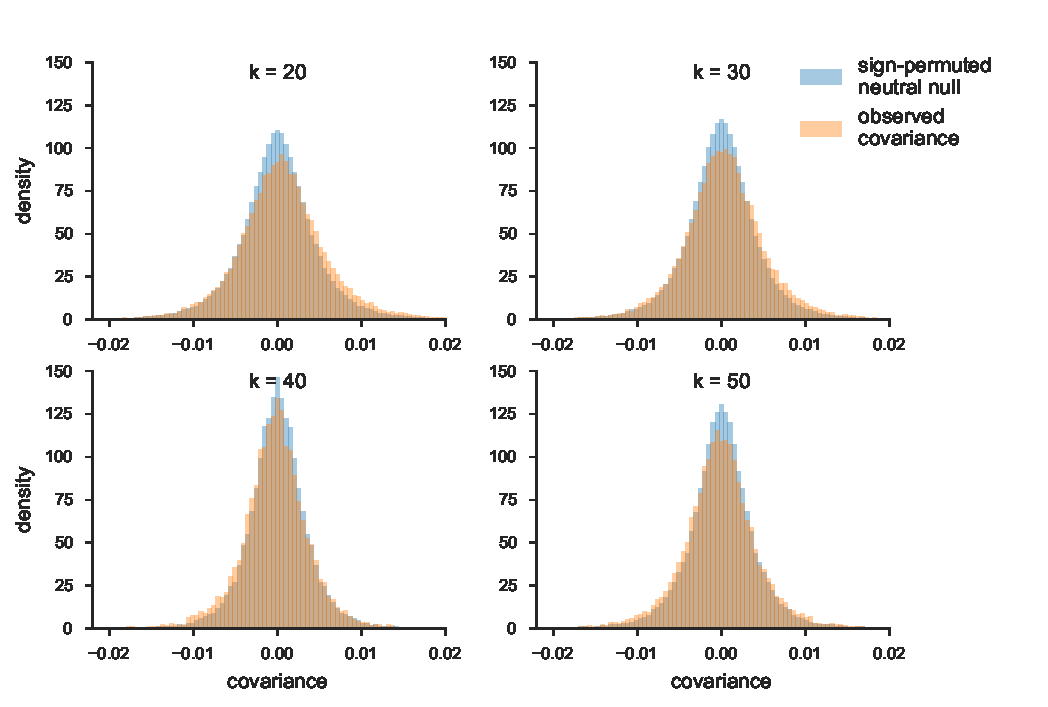
\includegraphics[]{figures/barghi-offset-panels.pdf}

  \caption{The distribution of temporal covariances calculated across 100kb
    genomic windows from \textcite{Barghi2019-qy}'s study (orange) and the
    block sign permuted empirical neutral null distribution of the windowed
    covariances (blue). Each panel shows these windowed covariances and the
    empirical null distribution for covariances $\cov(\Delta p_t, \Delta p_{t+k})$,
  $k$ is the number of generations between allele frequency changes.}
  \label{suppfig:barghi-empnull-tilecovs}
\end{figure}


\clearpage
\subsection{\textcite{Barghi2019-qy} Tail Probabilities for Windowed Covariances Distributions}

\begin{figure}[!ht]
  \centering
  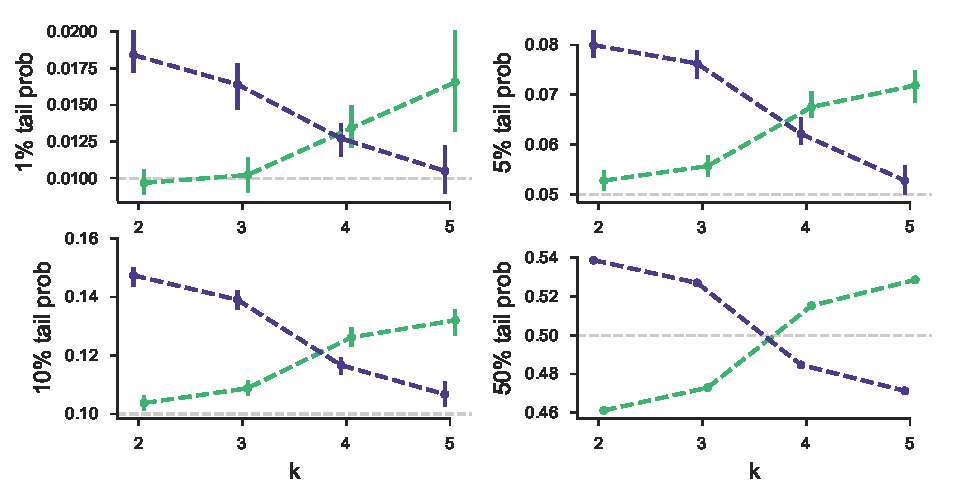
\includegraphics[]{figures/barghi-tailprobs-panels.pdf}

  \caption{\textcite{Barghi2019-qy} tail probabilities compared to
  sign-permuted empirical null distribution for various $\alpha$ levels.}

  \label{suppfig:barghi-tailprobs-panels}
\end{figure}

\begin{figure}[!ht]
  \centering

  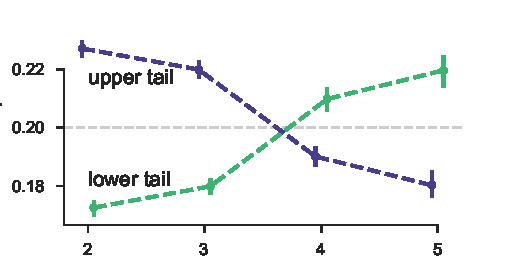
\includegraphics[]{figures/barghi-tailprobs-seqid-20.pdf}

  \caption{The 20\% lower and upper tail probabilities for the observed
    windowed covariances from the \textcite{Barghi2019-qy} study, based on
    sign-permuting at the chromosome level. This permutation empirical null is
    robust to long-range linkage disequilibrium acting over entire chromosomes
  (see Supplementary Material section \ref{supp:empirical-null}).}
  
  \label{suppfig:barghi-tailprobs-seqid}
\end{figure}


\end{document}
